\chapter{Memorie e Parallelismo}

\section{Memorie}
Un componente fondamentale di un processore è la \textbf{memoria}. Si implementa utilizzando dei registri da $ n $ bit (dette parole). Vogliamo realizzare una memoria il cui accesso sia simile ad un array nel linguaggio C. Ovvero vogliamo avere un vettore di registri a cui possiamo accedere con un offset intero. Data una memoria $ A $ si accederà alla parola $ k-esima $ tramite $ A[k] $. Per implementare tale selezione si può utilizzare un multiplexer che riceve in input le uscite dei singoli registri. I singoli registri ricevono tutti un segnale di clock in input, e permettono la scrittura attraverso un demultiplexer (decoder) che dato un indirizzo invia un 1 all'enable del registro selezionato. Si può mettere in AND il segnale enable del decoder insieme ad un input enable generale.

L'implementazione reale delle memorie (in particolare memorie flash), avviene ponendo delle linee dette "di parola" (orizzontali) e linee dette "bit line" (verticali) in una matrice.
All'incrocio delle linee vi è un condensatore. Il condensatore mantiene una carica per un breve periodo di tempo. Ho modo di controllare se nel condensatore alla posizione $ xy $ era "ricordato" un valore 1, mandando della corrente lungo la "linea di parola" $ x $. Se il condensatore era carico esso si scarica lungo la linea "bit line" $ y $. Inviando della corrente sulla linea di parola $ x $ leggeremo quindi dalle bit line (in alcuni casi indicate come source lines in output) la parola $ x $.
Prima di un condensatore, si inserisce un transistor nella giunzione fra WL e BL. Utilizzando un condensatore, nelle RAM dinamiche (Dynamic Random Access Memory) possono insorgere problemi dovuti ai tempi di carica e scarica del condensatore. Una volta letto un valore su una Bit Line, il condensatore si scarica e "perde" il valore precedentemente "ricordato".

\centerfig{0.65}{flashmem}{Memoria Flash}

Per selezionare la Word Line utilizziamo sempre un demultiplexer (decoder) che riceve un indirizzo. Nelle ram DDR comuni sono presenti spesso 8 o 9 chip. Ad esempio, su uno stick di ram DDR3 da 1GB (1 Giga Byte) sono presenti 8 memorie da 1Gb (1 Giga Bit), e generalmente anche una nona memoria che ricorda la "parità" per il controllo degli errori. Le RAM dinamiche perdono il loro contenuto se non sono alimentate. Visto il comportamento dei condensatori (la loro carica si perde lentamente) le DRAM hanno bisogno di un \textbf{refresh} periodico. Le DRAM sono molto economiche (1 transistor per 1 bit) ma possono risultare più lente rispetto alle alternative SRAM. Le memorie SRAM (Static RAM) sono meno economiche ma più rapide rispetto alle DRAM. Utilizzano flip-flop invece dei condensatori e per ogni bit utilizzano 6 transistor. Le memorie all'interno del processore (calcolatore) sono memorie statiche (realizzate con flip-flop) molto rapide. Un meccanismo sia a livello hardware che a livello di S.O. permette la suddivisione dei dati processati fra vari livelli di cache, dalla memoria statica del processore alla più capiente ma lenta DRAM.

\centerfig{0.35}{dramcell}{Schema di una cella di una memoria DRAM}

\begin{defn}
	\textbf{RAM, ROM, PROM e EEPROM:}
	L'acronimo RAM (Random Access Memory) indica in generale delle memorie sulle quali possiamo leggere e scrivere. Le memorie ROM sono memorie a sola lettura (Read Only Memory). Le memorie ROM non hanno condensatori nelle giunzioni della matrice, ma a momento di produzione vengono "incisi" dei collegamenti o isolamenti nelle giunzioni fra Word Line e Bit Line.
	Le memorie \textbf{PROM} utilizzano dei fusibili nelle giunzioni fra WL e BL per permettere agli acquirenti di scrivere nella memoria una volta sola. Di fabbrica tutti i bit di una PROM sono impostati a 1. Bruciando i fusibili nelle giunzioni si interrompono i collegamenti realizzando una vera e propria scrittura permanente. 
	
	\centerfig{0.65}{prom}{Esempio di memoria PROM}
	
	Un altro tipo di memorie sono le \textbf{EEPROM} (Electrically Erasable ROM). Utilizzano dei transistor particolari che possono essere "reimpostati" permettendo di cancellare e riscrivere la memoria con una corrente maggiore.
	
	Nella seconda parte del corso vedremo dettagliatamente Assembly ARM. Le istruzioni Assembly eseguono delle operazioni sui registri interni alla CPU.
	Un esempio di istruzione banale è la somma di numeri fra registri. \verb|ADD R1 R2 R3|. Nell'Assembly ARM la lettura avviene da destra a sinistra, ed il risultato viene memorizzato nel registro più a sinistra, in questo caso \verb|R1|.	
\end{defn}



\paragraph{Memorie Multi Porta e Tempi di Accesso}
Le memorie multiporta permettono la lettura parallela di due o più registri. Invece di un singolo multiplexer per leggere un registro, alle uscite dei registri è collegato un altro multiplexer che ricevendo un indirizzo diverso dal primo multiplexer, permette di leggere un altro valore dalla memoria, abilitando alla lettura parallela di due registri contemporaneamente. È fondamentale avere una memoria con almeno due porte per eseguire istruzioni su due registri alla volta. Indichiamo i tempi di accesso alla memoria con $ T_a $. Ad oggi siamo in un range di tempi inferiori ad un nanosecondo per i tempi di accesso ai flip-flop (poche decine di picosecondi), sull'ordine dei nanosecondi per le SRAM (cache) e sull'ordine dei microsecondi per le DRAM.


\centerfig{0.75}{DRAM512}{Modulo RAM Corsair DDR2-533}

\paragraph{Blocco memoria}
Introduciamo un blocco per la memoria da utilizzare nei diagrammi dei circuiti.
La memoria riceve in input un dato $ x $ da scrivere nell'indirizzo indicato dall'input di controllo \textbf{Address}. Se il segnale \textbf{enable} è HIGH allora avviene la scrittura di $ x $ all'interno dell'indirizzo puntato. Altrimenti, se \textbf{enable} è LOW avviene la lettura. Assumiamo che l'uscita sia stabile per il ciclo di clock
\diagram{memoryblock.tex}{Blocco Memoria}

\paragraph{LUT (Lookup Table)}
Una rete combinatoria che riceve $ n $ bit in input può essere implementata con una memoria ROM. Data una tabella di verità di una rete combinatoria, si può portare la tabella di verità in forma vettoriale per creare una LUT.
Una LUT o \textbf{Lookup Table} è in generale un array che rimpiazza una computazione, possibilmente complessa, con un operazione di accesso, nel caso delle reti combinatorie con una memoria ROM.
I bit in input della tabella di verità vengono portati a bit rappresentanti l'indirizzo di accesso della memoria, e i risultati della tabella di verità saranno memorizzati in un vettore di $ 2^n $ elementi (se la tabella di verità ha un solo output). 
Per quanto alcune reti combinatorie possono risultare più complesse a livello di circuito se implementate con una LUT, un vantaggio non banale delle Lookup Tables è che possono essere riprogrammate se viene utilizzata una memoria EEPROM. Ciò svolge un ruolo fondamentale negli FPGA. Le LUT possono essere utilizzate in parallelo.

\begin{exmp}
	\textbf{Rete Sequenziale di un contatore}
	Se volessimo realizzare un contatore, con le sole operazioni di incremento e decremento con un ASF, dovremmo avere un numero di stati pari alla capacità massima del contatore.
	Per realizzare un contatore sono necessari un registro da $ n $ bit, (prendiamo ad esempio 8 bit) ed una ALU che fa due sole operazioni (+1 e -1), quindi con un solo bit di controllo. Scegliamo se aumentare o decrementare il contatore impostando il bit di controllo della ALU, e scegliamo se scrivere nel prossimo ciclo di clock impostando ad HIGH il bit Enable (Event) del registro. Essendo una rete sequenziale, la funzione $ \sigma $ è implementata dalla ALU, e la funzione $ \omega $ è semplicemente l'identità. È una rete di Moore poiché la funzione identità non dipende dagli ingressi (Inc/Dec ed Event).
	
	\diagram{counter.tex}{Rete sequenziale di un contatore}
\end{exmp}


\begin{exmp}
	\textbf{Semplice Calcolatrice}
	Vogliamo realizzare una calcolatrice molto semplice da 32 bit per eseguire addizione, sottrazione, moltiplicazione e divisione. La calcolatrice riceverà in input due numeri $ A,B $ e restituirà in output il risultato, che potrà essere re-inserito nei due registri contenenti $ A $ e $ B $. Essa è una rete sequenziale che possiamo inserire in un componente che avrà in input i due numeri $ A,B $, la selezione dei due multiplexer per gli input, segnali di enable per la scrittura nel registro $ A $ e nel registro $ B $ e due bit di controllo per selezionare l'operazione. In output avrà il numero in uscita e 4 bit di flag (Overflow, Carry, Negative e Zero). Definiamo questa parte del calcolatore "parte operativa". Abbiamo bisogno anche di una "parte di controllo" che dati due input si occuperà di controllare le entrate di controllo della parte operativa della calcolatrice.
	
	\diagram{calculator.tex}{Semplice Calcolatore (Omesso clock per semplicità del disegno, è presente)}
\end{exmp}


\begin{defn}
	\textbf{if-then-else:}
	Supponiamo di voler realizzare un importante costrutto per la programmazione (\textit{if-then-else}) utilizzando solo componenti standard. Abbiamo due reti combinatorie $ f,g $, una parola memorizzata in un registro $ A $ e un registro $ B $ in cui sarà memorizzato il risultato. Vogliamo costruire una rete per evaluare l'espressione:
	
	\begin{Verbatim}
	if(expr) then
		g(A) -> B
	else
		f(A) -> B
	\end{Verbatim}
	
	\diagram{ifthenelse.tex}{Rete che implementa if-then-else}
\end{defn}

\begin{defn}
	\textbf{while:}
	Se volessimo invece implementare un ciclo while della forma:
	\begin{Verbatim}
	while(expr) do
	f(A) -> A
	\end{Verbatim}
	Possiamo realizzarlo con la seguente rete:
	
	\diagram{while.tex}{Rete che implementa while}
	
	In maniera simile è possibile realizzare anche un costrutto switch-case.
	Icarus Verilog, per trasformare programmi Verilog di moduli behavioural in netlist di componenti di reti logiche utilizza meccanismi simili.
\end{defn}

\begin{exrc}
	\textbf{Confronto maggiore}
	
	Vediamo ora diversi metodi per realizzare una rete combinatoria che controlla se un numero è maggiore di un altro, utile per realizzare operazioni condizionali.
	
	\includecode[verilog]{./verilog/confrontomaggiore/maggioreb.v}{Esercizio di confronto maggiore in Verilog (approccio algoritmico)}
	
	\FloatBarrier	
\end{exrc}


\subsection{Calcolatrice con registri di memoria}
Realizziamo adesso una calcolatrice con sottrazione e addizione che permette di leggere due numeri in input e fare operazioni utilizzando anche numeri precedentemente memorizzati in degli altri registri. Abbiamo bisogno di risorse di calcolo (una ALU) e registri o memorie. Abbiamo bisogno di una memoria multiporta particolare per realizzare correttamente il circuito. Questa memoria accetta 3 indirizzi, i primi due sono per la lettura (ha due parole in output) e il terzo indirizzo è per la scrittura. È una rete sequenziale, per questo motivo abbiamo bisogno di un meccanismo per evitare i problemi di temporizzazione. Essendo una rete sequenziale il tempo di esecuzione sarà $ \tau = \delta + \max\{t_\sigma, t_\omega\} $. Dovremmo prendere un tempo del ciclo di clock $ \tau = \delta + \max \left\{\begin{matrix}
t_\text{MUX} + t_\text{ALU}, \\
t_\text{ALU} + t_\text{MUX}
\end{matrix}\right\} $ dove $ t_\sigma = t_\text{MUX} + t_\text{ALU} $ e $ t_\omega = t_\text{ALU} + t_\text{MUX} $

\diagram{calculatormemory.tex}{Calcolatrice con memoria.}

%//TODO codice verilog

\section{Parallelismo}

\begin{defn}
	
	Supponiamo di avere una serie di libri $ L_1, L_2, L_3, L_4 $ da tradurre. Vogliamo ridurre il tempo totale di traduzione di tutti i libri. Se a tradurre un libro impiego un tempo da $ t_0 $ a $ t_1 $, suddividendo la traduzione a metà fra due persone, impiegheremo $ t_{1/2} $ a tradurre il libro. L'obiettivo del parallelismo è ridurre la \textbf{latenza}. Se ho un insieme di libri, la latenza $ L $ di un libro è il tempo necessario per tradurlo (il tempo a cui ho terminato la traduzione, meno il tempo in cui ho iniziato la traduzione). Se ho $ m $ task da completare, il \textbf{tempo di completamento}  $ T_c = m \cdot L$ è il tempo totale necessario a completare tutti i task m. Con il parallelismo vogliamo diminuire il tempo di completamento. Con \textbf{tempo di servizio} intendiamo l'intervallo medio di tempo fra la "consegna" di due risultati successivi. Definiamo anche \textbf{throughput} come il numero di calcoli eseguiti per unità di tempo.
	
	Data una lista di istruzioni $ i_0, i_1, i_2, i_3, \dots $ il nostro processore esegue (in pseudocodice):
	
	\begin{lstlisting}
	while(true) {
	leggi un istruzione (ASM)
	interpreta
	esegui
	}
	\end{lstlisting} 
\end{defn}


\begin{defn}
	\textbf{Tempo ideale:}
	Dato $ n = $ numero di worker (o grado di parallelismo) e $ T_{\text{seq}} = $ il tempo sequenziale, il \textbf{tempo ideale} $ T_{\text{id}}(n) = \dfrac{T_{\text{seq}}}{n}$.
\end{defn}


\begin{defn}
	\textbf{Speedup:}
	Definiamo anche lo \textbf{speedup} come $ \dfrac{T_{\text{seq}}}{T(n)} $, ovvero il miglior tempo sequenziale fratto il tempo parallelo con grado di parallelismo $ n $.
\end{defn}

\begin{defn}
	\textbf{Scalabilità:} $ \text{Scalab}(n) = \dfrac{T(1)}{T(n)} \leq n $
\end{defn}

\begin{defn}
	\textbf{Efficienza:}
	$ \text{Efficienza}(n) = \dfrac{T_{\text{id}}}{T(n))} = \dfrac{T_{\text{seq}}/n}{T(n)} = \dfrac{T_{\text{seq}}}{n \cdot T(n)} \leq 1 $
\end{defn}


\begin{defn}
	\textbf{Parallelismo temporale o Pipelining:} Il processore deve sempre eseguire dei task (istruzioni) sequenzialmente per eseguire un programma, e si può diminuire la latenza dei singoli task per ridurre il tempo di esecuzione del programma.
	
	\centerfig{0.75}{pipelining}{Diagramma temporale del pipelining di una CPU.}
	
	Avremo che $ T_c = $ tempo iniziale di "riempimento" della pipeline + tempo $ ( \propto ( m \cdot $ tempo delle singole istruzioni )) 
	
	In alternativa, il nostro processore può assegnare un "ciclo" ad ogni istruzione
	
	\begin{lstlisting}[frame=single]
	// Per istruzione 0
	while(true) {
	leggi, decodifica, esegui
	}
	\end{lstlisting} 
	\begin{lstlisting}[frame=single]
	// Per istruzione 1
	while(true) {
	leggi, decodifica, esegui
	}
	\end{lstlisting} 
	\begin{lstlisting}[frame=single]
	// Per istruzione 2...
	while(true) {
	leggi, decodifica, esegui
	}
	\end{lstlisting} 
	
	\centerfig{0.75}{pipelining2}{Pipelining con più worker (parallelismo temporale).}
	
	Usando il \textbf{parallelismo temporale}, ad ogni periodo $ L $ otterremo 3 risultati. Ciò riduce il tempo di servizio a $ \frac{1}{3}L $. Le istruzioni dei task sono comunque eseguite sequenzialmente su worker separati.	
\end{defn}



\begin{defn}
	\textbf{Parallelismo spaziale:}
	Nel \textbf{parallelismo spaziale}, suddividiamo le istruzioni di ogni task su worker diversi. Significa che i worker possono eseguire in parallelo le istruzioni di un singolo task. Il parallelismo spaziale serve a diminuire la latenza, il parallelismo temporale serve invece ad aumentare il throughput.
	
\end{defn}

%//TODO diagramma memorie parallellismo dei moduli di memoria multiplexer 18 ottobre 11:55, togliere multiplexer per parallelizzare.

%//TODO diagramma differenza pipeline - farm - map

\paragraph{Pipeline (stream parallel)}

%//TODO diagramma pipeline

Avendo 3 worker ed eseguendo 3 istruzioni a cascata che impiegano rispettivamente $ 2t, 3t, 1t $, se eseguiamo dei task successivamente, le istruzioni dei task successivi avverrano con un delay dovuto alla differenza del tempo di esecuzione. Dopo un numero di istruzioni le istruzioni si sincronizzeranno. Se i worker impiegano rispettivamente dei tempi $ t_1,t_2,t_3 $, il tempo di completamento di $ m $ istruzioni sarà $ T_c = \sum t_i + m \cdot \max\{t_1,t_2,t_3\} $. Ciò crea una situazione non ottimale

\[ \begin{aligned}
n = \text{numero di stadi della pipeline} \\
T_s = \max\{T_{Si}\} \\
\max(\text{speedup(n)}) = \text{\# di stadi della pipeline} \\
T_c (n) = \sum_i L_i + n-1 T_s
\end{aligned} \]

\centerfig{0.75}{nopipeline}{Processore senza pipeline (sottoscalare)}
\centerfig{0.75}{fivestagespipeline}{Processore con pipeline a cinque stadi (scalare)}
\centerfig{0.75}{Superscalarpipeline}{Processore con pipeline superscalare}

\paragraph{Map e Farm}

% //TODO diagramma map 
Farm è di tipo \textit{stream parallel} mentre map è di tipo \textit{data parallel}. Nel caso del \textbf{Map} (e anche del Farm), se le  istruzioni impiegano un tempo $ t $ che viene precisamente suddiviso in $ t/2 $ allora il problema non sussiste. Se invece vengono suddivise in tempi diversi si creano spazi temporali in cui non è possibile sfruttare tutta la potenza di calcolo. Nella map posso suddividere un dato in arrivo e fare del calcolo in parallelo su di esso (\textit{data parallelism}). Nella farm e nella pipeline i dati in arrivo possono essere passati a diversi worker (verrano schedulati) che eseguono computazioni in parallelo (\textit{stream parallelism}). I dati non possono essere suddivisi nello \textit{stream parallelism} come nel \textit{data parallelism}.

\paragraph{Tempi della Farm}
\[ \begin{aligned}
nw = \text{grado di parallelismo}\\
T_w = \text{ il tempo che 1 worker impiega per calcolare 1 risultato} \\
T_s = \max\left\{T_{\text{sched}}, \dfrac{T_w}{nw}, T_{\text{coll}}\right\}
\end{aligned} \]

\paragraph{Tempi della Map}
\[ \begin{aligned}
T_c = T_\text{split} + \dfrac{m}{nw} T_f + T_\text{merge} \\
T_s = \max\left\{T_\text{split}, T_\text{merge}, \dfrac{m}{nw}t_f\right\}
\end{aligned} \]

\subsection{Processore superscalare}

Scriviamo un loop di esecuzione del processore in maniera più accurata.

\begin{lstlisting}[frame=single]
while(true) {
I = fetch(PC) // PC = program counter
decode(I)
exec(I)
|--> update(PC)
}
\end{lstlisting}

% //TODO diagramma program counter modulo di memoria sopra, pipeline sotto e superscalare

% //TODO diagramma esempio libro

\paragraph{Composizione nel parallelismo}

Possiamo comporre i diversi metodi di parallelismo. Ad esempio si può realizzare una pipeline che contiene una farm. Prendiamo ad esempio

\[ \begin{aligned}
\text{pipe}(S_1, \text{farm}(S_2), S_3) \\
\text{Un possibile schema dei worker della pipeline è} \\
\to f \to \begin{cases}
\text{(farm)} \\
g \\ g
\end{cases} \to h \\
\text{Calcoliamo i tempi} \\
T_s = \max\left\{T_{S_1}, T_{S_2}, T_{S_3}\right\} \\
T_s = \max\left\{T_f, \max\left\{T_\text{sched}, \dfrac{T_g}{nw}, T_\text{coll}\right\}, T_h \right\} \\
= \max\left\{T_f, T_\text{sched}, \dfrac{T_g}{nw}, T_\text{coll}, T_h \right\}
\end{aligned} \]

% //TODO maggiore tabella e normale

\begin{defn}
	\textbf{Bottleneck o Colli di Bottiglia}
	
	Supponiamo di avere due computazioni composte $ f \circ g $. Se $ f $ impiega $ 5t $ e $ g $ impiega $ 2t $, eseguire in successione $ \to f \to g \to $ può causare dei bottleneck (rallentamenti). Se $ f $ è data parallel si può suddividere la sua computazione in parti uguali (ad esempio due) e poi passare il risultato a $ g $. In alternativa si può dividere $ f $ in 5 parti uguali e ad ogni parte calcolare la composizione sequenziale (in una farm) in modo che $ T_s = \max\left\{T_\text{sched}, \dfrac{T_w}{nw}, T_\text{coll}\right\} \approx \dfrac{Tw}{nw} \approx \dfrac{7t}{5} \approx 1$

	% //TODO diagramma bottleneck
\end{defn}

\begin{exmp}
	\textbf{Pipeline in Verilog}
	
	Vediamo adesso una pipeline per parallelizzare l'operazione di moltiplicazione per 2 composta due volte.
	
	
	\includecode[verilog]{./verilog/2xpipeline/singlestage/per2.v}{Modulo moltiplicazione per 2}
	\includecode[verilog]{./verilog/2xpipeline/singlestage/per4.v}{Modulo moltiplicazione per 4}
	\includecode[verilog]{./verilog/2xpipeline/singlestage/test.v}{Programma di test}
	
	\includecode[verilog]{./verilog/2xpipeline/twostages/per2.v}{Modulo moltiplicazione per 2 (pipelined)}
	\includecode[verilog]{./verilog/2xpipeline/twostages/per4.v}{Modulo moltiplicazione per 4 (pipelined)} 
	\includecode[verilog]{./verilog/2xpipeline/twostages/test.v}{Programma di test (pipelined)}
	
	%//TODO immagine gtkwave
\end{exmp}

\section{Homework}

\begin{exrc}
	Si forniscano le espressioni booleane che calcolano:
	Se una configurazione di 8 bit è una potenza di due: È necessario soltanto uno XOR dei singoli bit $ b_0 \oplus b_1 \oplus b_2 \oplus b_3 \oplus b_4 \oplus b_5 \oplus b_6 \oplus b_7 \oplus $.
	
	Fornire le espressioni booleane che calcolano l'indice del bit più significativo a 1 in una configurazione di 8 bit: 
	\begin{table}[H]
		\centering
		\caption{Tabella di verità di una rete combinatoria che restituisce l'indice del bit più significativo a 1 di una configurazione di 8 bit. L'indice inizia da 1, il valore in output 0 viene usato se il numero in input sono tutti 0}
		\label{tab:homework1}
		\begin{tabular}{|llllllll|llll|}
			\hline
			$x_7$ & $x_6$ & $x_5$ & $x_4$ & $x_3$ & $x_2$ & $x_1$ & $x_0$ & $z_3$ & $z_2$ & $z_1$ & $z_0$ \\ \hline
			1     & -     & -     & -     & -     & -     & -     & -     & 0     & 1     & 1     & 1     \\ \hline
			0     & 1     & -     & -     & -     & -     & -     & -     & 0     & 1     & 1     & 0     \\ \hline
			0     & 0     & 1     & -     & -     & -     & -     & -     & 0     & 1     & 0     & 1     \\ \hline
			0     & 0     & 0     & 1     & -     & -     & -     & -     & 0     & 1     & 0     & 0     \\ \hline
			0     & 0     & 0     & 0     & 1     & -     & -     & -     & 0     & 0     & 1     & 1     \\ \hline
			0     & 0     & 0     & 0     & 0     & 1     & -     & -     & 0     & 0     & 1     & 0     \\ \hline
			0     & 0     & 0     & 0     & 0     & 0     & 1     & -     & 0     & 0     & 0     & 1     \\ \hline
			0     & 0     & 0     & 0     & 0     & 0     & 0     & 1     & 0     & 0     & 0     & 0     \\ \hline
			0     & 0     & 0     & 0     & 0     & 0     & 0     & 0     & 1     & 1     & 1     & 1     \\ \hline
		\end{tabular}
	\end{table}

	\begin{equation*}
		\begin{aligned}
		z_3 = \overbar{x_7x_6x_5x_4x_3x_2x_1x_0} \\
		z_2 = x7 + \overbar{x_7}x_6 + \overbar{x_7x_6}x_5 + \overbar{x_7x_6x_5}x_4 + \overbar{x_7x_6x_5x_4x_3x_2x_1x_0} \\
		z_1 = x7 + \overbar{x_7}x_6 + \overbar{x_7x_6x_5x_4}x_3 + \overbar{x_7x_6x_5x_4x_3}x_2 + \overbar{x_7x_6x_5x_4x_3x_2x_1x_0} \\
		z_0 = x7 + \overbar{x_7x_6}x_5 + \overbar{x_7x_6x_5x_4}x_3 + \overbar{x_7x_6x_5x_4x_3x_2}x_1 + \overbar{x_7x_6x_5x_4x_3x_2x_1}x_0 \\
		\end{aligned}
	\end{equation*}
\end{exrc}

\begin{exrc}
	Delle reti combinatorie definite dalle espressioni booleane dell’esercizio precedente si fornisca l’implementazione come module Verilog insieme ad un programma testbench che ne dimostri il corretto funzionamento.
	
	Per calcolare se un numero è potenza di due non utilizziamo il bitwise xor, ma mettiamo in bitwise AND il numero in input e il numero in input a cui sottraiamo 1. Se il numero in input è una potenza di due, quando gli viene sottratto 1 rimarrano soltanto 1 a destra della posizione dell'1 nel numero in input. Se l'AND è 0 allora il numero è potenza di due.

	\includecode[verilog]{./verilog/homework/potenzadidue/potenzadidue.v}{Modulo che calcola se una configurazione di bit è potenza di 2}
	
	\includecode[verilog]{./verilog/homework/potenzadidue/test.v}{Modulo di test della rete combinatoria che calcola se una configurazione di bit è potenza di 2}
	
	\centerfig{0.8}{potenzadiduegtkwave.png}{Visualizzazione dell'esecuzione del modulo che calcola se un numero da 8 bit è potenza di 2}
	
	Per implementare una rete combinatoria che restituisce l'indice del bit più significativo si può utilizzare un semplice ciclo for per realizzare un modulo behavioral. La funzione built-in \verb|$clog2()| calcola il logaritmo in base 2 di un numero. La utilizziamo per definire la dimensione dell'output del modulo, dato che il numero di bit $ n $ del valore in input è rappresentabile con un numero di $ \log_2(n) $ bit.
	
	\includecode[verilog]{./verilog/homework/indice/index.v}{Modulo della rete combinatoria che calcola l'indice del bit ad 1 più significativo in un numero da N bit}
	
	\includecode[verilog]{./verilog/homework/indice/test.v}{Modulo di test del modulo che calcola l'indice del bit ad 1 più significativo in un numero da N bit}
	
	\centerfig{0.85}{indexgtkwave}{Visualizzazione dell'esecuzione del modulo di test del modulo che calcola l'indice del bit ad 1 più significativo in un numero da N bit}
	
\end{exrc}

\begin{exrc}
	Definire un automa che processa una coppia di variabili da k bit e che conta, modulo 2, il numero delle volte che le due variabili in ingresso sono uguali.
	
	\begin{figure}[H]
		\centering
		\caption{Automa di Moore che conta quante volte gli input sono uguali. Gli stati possono essere teoricamente infiniti, l'output è uguale al numero di stato, realisticamente gli stati possibili saranno $ 2^n $ dove $ n $ è il numero di bit nel registro}
		\begin{tikzpicture}[->,>=stealth',shorten >=1pt,auto,node distance=3.5cm]
		
		\node[state,initial] 	(1)                   		{1};
		\node[state]         	(2) [right of=1] 	   		{2};
		\node[state]         	(3) [right of=2] 	   		{3};
		\node[state]         	(4) [right of=3] 	   		{$\hdots$};
		
		\path 	
		(1)		edge [bend left]  	node {$x = y$} 		(2)
				edge [loop below] 	node {$x \neq y$} 	(1)
		(2) 	edge [loop below] 	node {$x \neq y$} 	(2)
				edge [bend left] 	node {$x = y$} 		(3)
		(3)		edge [loop below]  	node {$x \neq y$} 	(3)
				edge [bend left]  	node {$x = y$} 		(4);
		\end{tikzpicture}
	\end{figure}
	
	Per semplicità di implementazione in Verilog decidiamo di utilizzare un contatore come registro. (L'alternativa potrebbe essere includere una ALU nel modulo di $ \sigma $ che legge il valore del registro di stato e lo incrementa di uno nel caso lo stato debba essere incrementato).
	La funzione $ \sigma $ calcolerà $ x \mod 2 $ e $ y \mod 2 $, eseguirà un confronto e nel caso siano uguali invierà il risultato del confronto alla linea \verb|INCREMENT| del contatore, così che al prossimo ciclo di clock il contatore delle volte che $ x $ e $ y $ sono uguali aumenti. La funzione $ \omega $ è la funzione identità.
\end{exrc}

\begin{exrc}
	Implementare l'automa dell'esercizio precedente in Verilog.
	
	\includecode[verilog]{./verilog/homework/contauguali/counter.v}{Modulo contatore}
	
	\includecode[verilog]{./verilog/homework/contauguali/sigma.v}{Modulo di $ \sigma $ che controlla se $ x $ e $ y $ sono uguali modulo 2 e invia il bit di increment al contatore}
	
	\includecode[verilog]{./verilog/homework/contauguali/test.v}{Modulo di test della rete combinatoria dell'automa che conta il numero di volte che due numeri in input sono uguali modulo 2}
	
	\centerfig{0.8}{contaugualigtkwave.png}{Visualizzazione dell'esecuzione del modulo di test dell'automa che conta quante volte due numeri sono uguali modulo 2}
\end{exrc}

\begin{exrc}
	Progettare, utilizzando componenti standard una rete sequenziale che possa essere utilizzata per implementare operazioni di push e pop su uno stack di massimo 8 posizioni.
	
	\begin{figure}[H]
		\centering
		\scalebox{0.5}{% Graphic for TeX using PGF
% Title: /home/sea/uni/ae/appunti-ae-2019-arm/diagrams/homeworkstack.dia
% Creator: Dia v0.97.3
% CreationDate: Sun Oct 27 19:05:44 2019
% For: sea
% \usepackage{tikz}
% The following commands are not supported in PSTricks at present
% We define them conditionally, so when they are implemented,
% this pgf file will use them.
\ifx\du\undefined
  \newlength{\du}
\fi
\setlength{\du}{15\unitlength}
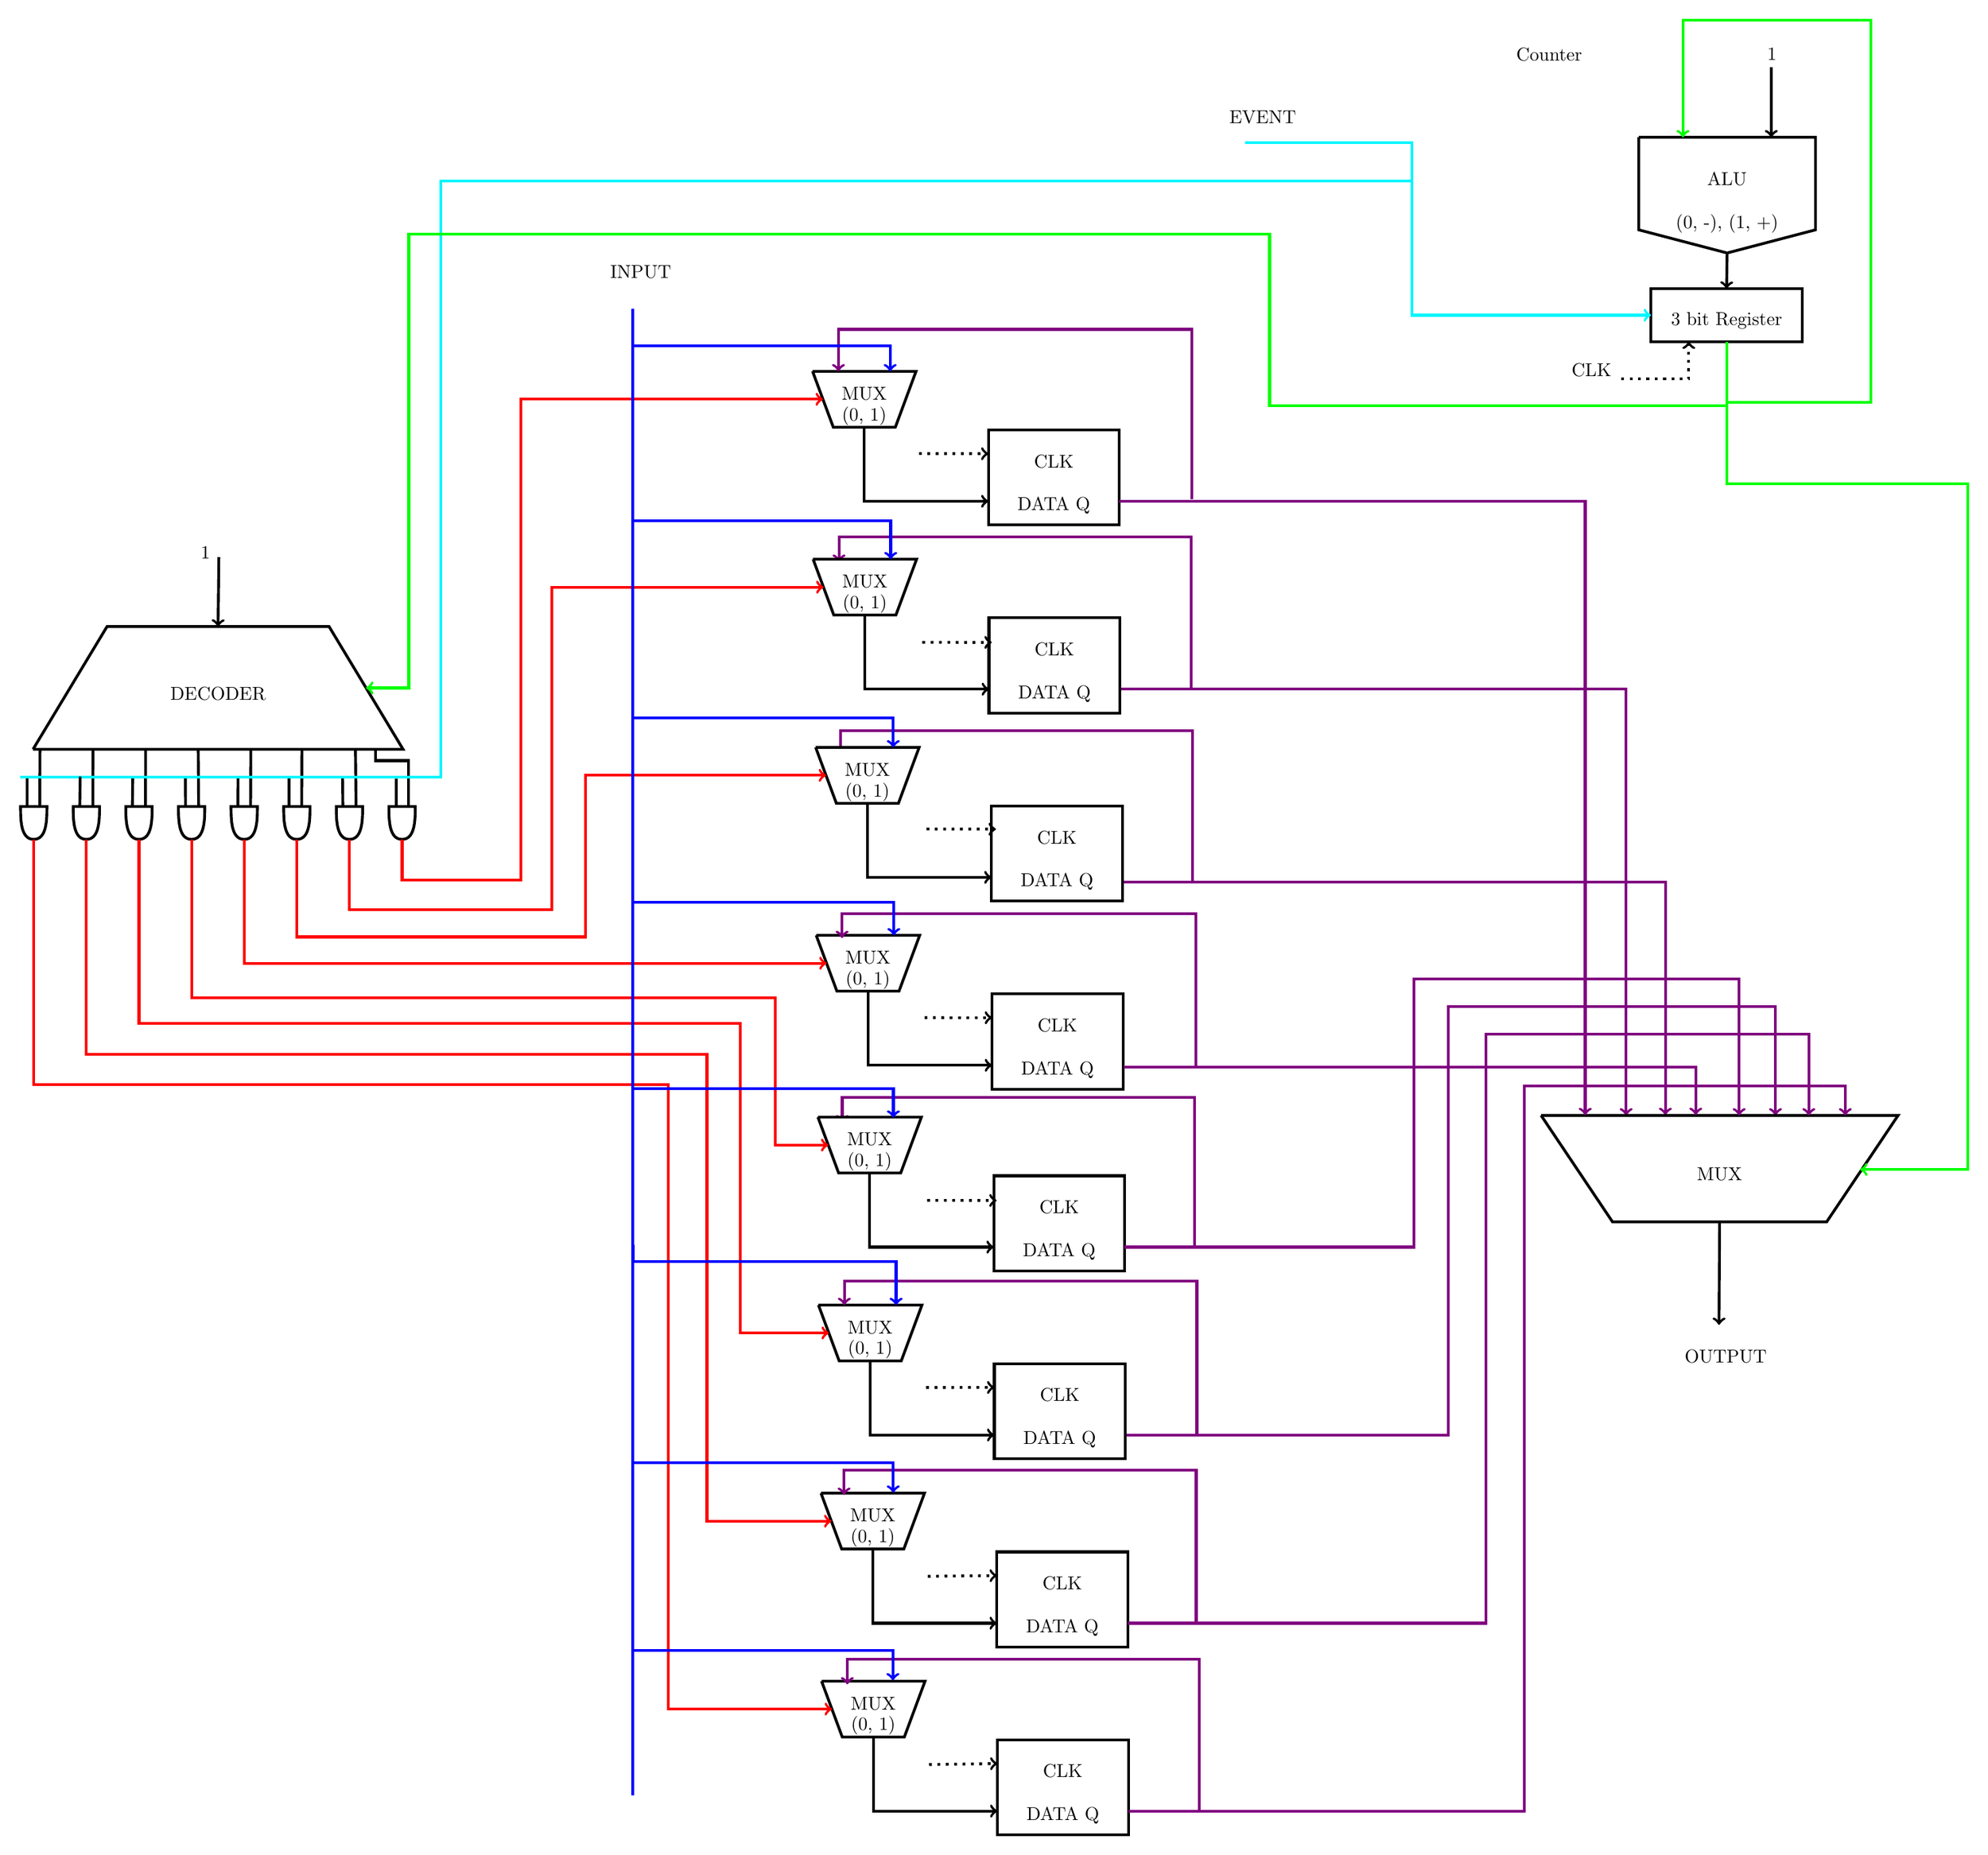
\begin{tikzpicture}
\pgftransformxscale{1.000000}
\pgftransformyscale{-1.000000}
\definecolor{dialinecolor}{rgb}{0.000000, 0.000000, 0.000000}
\pgfsetstrokecolor{dialinecolor}
\definecolor{dialinecolor}{rgb}{1.000000, 1.000000, 1.000000}
\pgfsetfillcolor{dialinecolor}
\pgfsetlinewidth{0.100000\du}
\pgfsetdash{}{0pt}
\pgfsetdash{}{0pt}
\pgfsetmiterjoin
\pgfsetbuttcap
{
\definecolor{dialinecolor}{rgb}{0.000000, 0.000000, 0.000000}
\pgfsetfillcolor{dialinecolor}
% was here!!!
{\pgfsetcornersarced{\pgfpoint{0.000000\du}{0.000000\du}}\definecolor{dialinecolor}{rgb}{0.000000, 0.000000, 0.000000}
\pgfsetstrokecolor{dialinecolor}
\draw (4.097910\du,25.783261\du)--(4.097910\du,24.143346\du)--(2.903967\du,24.143346\du)--(2.903967\du,23.648410\du);
}}
\pgfsetlinewidth{0.100000\du}
\pgfsetdash{}{0pt}
\pgfsetdash{}{0pt}
\pgfsetbuttcap
{
\definecolor{dialinecolor}{rgb}{0.000000, 0.000000, 0.000000}
\pgfsetfillcolor{dialinecolor}
% was here!!!
\definecolor{dialinecolor}{rgb}{0.000000, 0.000000, 0.000000}
\pgfsetstrokecolor{dialinecolor}
\draw (2.194608\du,23.730388\du)--(2.214329\du,25.783261\du);
}
\pgfsetlinewidth{0.100000\du}
\pgfsetdash{}{0pt}
\pgfsetdash{}{0pt}
\pgfsetbuttcap
{
\definecolor{dialinecolor}{rgb}{0.000000, 0.000000, 0.000000}
\pgfsetfillcolor{dialinecolor}
% was here!!!
\definecolor{dialinecolor}{rgb}{0.000000, 0.000000, 0.000000}
\pgfsetstrokecolor{dialinecolor}
\draw (1.735024\du,24.773290\du)--(1.742980\du,25.783261\du);
}
\pgfsetlinewidth{0.100000\du}
\pgfsetdash{}{0pt}
\pgfsetdash{}{0pt}
\pgfsetbuttcap
{
\definecolor{dialinecolor}{rgb}{0.000000, 0.000000, 0.000000}
\pgfsetfillcolor{dialinecolor}
% was here!!!
\definecolor{dialinecolor}{rgb}{0.000000, 0.000000, 0.000000}
\pgfsetstrokecolor{dialinecolor}
\draw (0.276729\du,23.698571\du)--(0.270131\du,25.745041\du);
}
\pgfsetlinewidth{0.100000\du}
\pgfsetdash{}{0pt}
\pgfsetdash{}{0pt}
\pgfsetbuttcap
{
\definecolor{dialinecolor}{rgb}{0.000000, 0.000000, 0.000000}
\pgfsetfillcolor{dialinecolor}
% was here!!!
\definecolor{dialinecolor}{rgb}{0.000000, 0.000000, 0.000000}
\pgfsetstrokecolor{dialinecolor}
\draw (-0.182855\du,24.741473\du)--(-0.183542\du,25.745041\du);
}
\pgfsetlinewidth{0.100000\du}
\pgfsetdash{}{0pt}
\pgfsetdash{}{0pt}
\pgfsetbuttcap
{
\definecolor{dialinecolor}{rgb}{0.000000, 0.000000, 0.000000}
\pgfsetfillcolor{dialinecolor}
% was here!!!
\definecolor{dialinecolor}{rgb}{0.000000, 0.000000, 0.000000}
\pgfsetstrokecolor{dialinecolor}
\draw (-1.552768\du,23.702106\du)--(-1.559366\du,25.748576\du);
}
\pgfsetlinewidth{0.100000\du}
\pgfsetdash{}{0pt}
\pgfsetdash{}{0pt}
\pgfsetbuttcap
{
\definecolor{dialinecolor}{rgb}{0.000000, 0.000000, 0.000000}
\pgfsetfillcolor{dialinecolor}
% was here!!!
\definecolor{dialinecolor}{rgb}{0.000000, 0.000000, 0.000000}
\pgfsetstrokecolor{dialinecolor}
\draw (-2.012351\du,24.745008\du)--(-2.013038\du,25.748576\du);
}
\pgfsetlinewidth{0.100000\du}
\pgfsetdash{}{0pt}
\pgfsetdash{}{0pt}
\pgfsetbuttcap
{
\definecolor{dialinecolor}{rgb}{0.000000, 0.000000, 0.000000}
\pgfsetfillcolor{dialinecolor}
% was here!!!
\definecolor{dialinecolor}{rgb}{0.000000, 0.000000, 0.000000}
\pgfsetstrokecolor{dialinecolor}
\draw (-3.435293\du,23.687965\du)--(-3.418740\du,25.765585\du);
}
\pgfsetlinewidth{0.100000\du}
\pgfsetdash{}{0pt}
\pgfsetdash{}{0pt}
\pgfsetbuttcap
{
\definecolor{dialinecolor}{rgb}{0.000000, 0.000000, 0.000000}
\pgfsetfillcolor{dialinecolor}
% was here!!!
\definecolor{dialinecolor}{rgb}{0.000000, 0.000000, 0.000000}
\pgfsetstrokecolor{dialinecolor}
\draw (-3.894877\du,24.730867\du)--(-3.890089\du,25.765585\du);
}
\pgfsetlinewidth{0.100000\du}
\pgfsetdash{}{0pt}
\pgfsetdash{}{0pt}
\pgfsetbuttcap
{
\definecolor{dialinecolor}{rgb}{0.000000, 0.000000, 0.000000}
\pgfsetfillcolor{dialinecolor}
% was here!!!
\definecolor{dialinecolor}{rgb}{0.000000, 0.000000, 0.000000}
\pgfsetstrokecolor{dialinecolor}
\draw (-5.317819\du,23.726853\du)--(-5.319998\du,25.747909\du);
}
\pgfsetlinewidth{0.100000\du}
\pgfsetdash{}{0pt}
\pgfsetdash{}{0pt}
\pgfsetbuttcap
{
\definecolor{dialinecolor}{rgb}{0.000000, 0.000000, 0.000000}
\pgfsetfillcolor{dialinecolor}
% was here!!!
\definecolor{dialinecolor}{rgb}{0.000000, 0.000000, 0.000000}
\pgfsetstrokecolor{dialinecolor}
\draw (-5.777403\du,24.769755\du)--(-5.791347\du,25.747909\du);
}
\pgfsetlinewidth{0.100000\du}
\pgfsetdash{}{0pt}
\pgfsetdash{}{0pt}
\pgfsetbuttcap
{
\definecolor{dialinecolor}{rgb}{0.000000, 0.000000, 0.000000}
\pgfsetfillcolor{dialinecolor}
% was here!!!
\definecolor{dialinecolor}{rgb}{0.000000, 0.000000, 0.000000}
\pgfsetstrokecolor{dialinecolor}
\draw (-7.200345\du,23.677359\du)--(-7.203580\du,25.783261\du);
}
\pgfsetlinewidth{0.100000\du}
\pgfsetdash{}{0pt}
\pgfsetdash{}{0pt}
\pgfsetbuttcap
{
\definecolor{dialinecolor}{rgb}{0.000000, 0.000000, 0.000000}
\pgfsetfillcolor{dialinecolor}
% was here!!!
\definecolor{dialinecolor}{rgb}{0.000000, 0.000000, 0.000000}
\pgfsetstrokecolor{dialinecolor}
\draw (-9.098239\du,23.736792\du)--(-9.104838\du,25.783261\du);
}
\pgfsetlinewidth{0.100000\du}
\pgfsetdash{}{0pt}
\pgfsetdash{}{0pt}
\pgfsetmiterjoin
\pgfsetbuttcap
{
\definecolor{dialinecolor}{rgb}{0.501961, 0.000000, 0.501961}
\pgfsetfillcolor{dialinecolor}
% was here!!!
\pgfsetarrowsend{to}
{\pgfsetcornersarced{\pgfpoint{0.000000\du}{0.000000\du}}\definecolor{dialinecolor}{rgb}{0.501961, 0.000000, 0.501961}
\pgfsetstrokecolor{dialinecolor}
\draw (32.238352\du,41.583495\du)--(32.238352\du,36.199982\du)--(19.617651\du,36.199982\du)--(19.617651\du,37.093133\du);
}}
\pgfsetlinewidth{0.100000\du}
\pgfsetdash{}{0pt}
\pgfsetdash{}{0pt}
\pgfsetmiterjoin
\pgfsetbuttcap
{
\definecolor{dialinecolor}{rgb}{0.501961, 0.000000, 0.501961}
\pgfsetfillcolor{dialinecolor}
% was here!!!
\pgfsetarrowsend{to}
{\pgfsetcornersarced{\pgfpoint{0.000000\du}{0.000000\du}}\definecolor{dialinecolor}{rgb}{0.501961, 0.000000, 0.501961}
\pgfsetstrokecolor{dialinecolor}
\draw (32.159845\du,28.533940\du)--(32.159845\du,23.066831\du)--(19.552812\du,23.066831\du)--(19.552812\du,23.959982\du);
}}
\pgfsetlinewidth{0.100000\du}
\pgfsetdash{}{0pt}
\pgfsetdash{}{0pt}
\pgfsetmiterjoin
\pgfsetbuttcap
{
\definecolor{dialinecolor}{rgb}{0.501961, 0.000000, 0.501961}
\pgfsetfillcolor{dialinecolor}
% was here!!!
\pgfsetarrowsend{to}
{\pgfsetcornersarced{\pgfpoint{0.000000\du}{0.000000\du}}\definecolor{dialinecolor}{rgb}{0.501961, 0.000000, 0.501961}
\pgfsetstrokecolor{dialinecolor}
\draw (32.108674\du,21.596855\du)--(32.108674\du,16.129746\du)--(19.501642\du,16.129746\du)--(19.501642\du,17.022897\du);
}}
\pgfsetlinewidth{0.100000\du}
\pgfsetdash{}{0pt}
\pgfsetdash{}{0pt}
\pgfsetmiterjoin
\pgfsetbuttcap
{
\definecolor{dialinecolor}{rgb}{0.501961, 0.000000, 0.501961}
\pgfsetfillcolor{dialinecolor}
% was here!!!
\pgfsetarrowsend{to}
{\pgfsetcornersarced{\pgfpoint{0.000000\du}{0.000000\du}}\definecolor{dialinecolor}{rgb}{0.501961, 0.000000, 0.501961}
\pgfsetstrokecolor{dialinecolor}
\draw (29.248834\du,48.286995\du)--(41.301380\du,48.286995\du)--(41.301380\du,32.950000\du)--(53.023050\du,32.950000\du)--(53.023050\du,36.845200\du);
}}
\pgfsetlinewidth{0.100000\du}
\pgfsetdash{}{0pt}
\pgfsetdash{}{0pt}
\pgfsetmiterjoin
\pgfsetbuttcap
{
\definecolor{dialinecolor}{rgb}{0.501961, 0.000000, 0.501961}
\pgfsetfillcolor{dialinecolor}
% was here!!!
\pgfsetarrowsend{to}
{\pgfsetcornersarced{\pgfpoint{0.000000\du}{0.000000\du}}\definecolor{dialinecolor}{rgb}{0.501961, 0.000000, 0.501961}
\pgfsetstrokecolor{dialinecolor}
\draw (29.548100\du,28.497600\du)--(49.082600\du,28.497600\du)--(49.082600\du,36.830100\du);
}}
\pgfsetlinewidth{0.100000\du}
\pgfsetdash{}{0pt}
\pgfsetdash{}{0pt}
\pgfsetmiterjoin
\pgfsetbuttcap
{
\definecolor{dialinecolor}{rgb}{0.501961, 0.000000, 0.501961}
\pgfsetfillcolor{dialinecolor}
% was here!!!
\pgfsetarrowsend{to}
{\pgfsetcornersarced{\pgfpoint{0.000000\du}{0.000000\du}}\definecolor{dialinecolor}{rgb}{0.501961, 0.000000, 0.501961}
\pgfsetstrokecolor{dialinecolor}
\draw (29.407234\du,21.584095\du)--(47.678425\du,21.584095\du)--(47.678425\du,36.845200\du);
}}
\definecolor{dialinecolor}{rgb}{1.000000, 1.000000, 1.000000}
\pgfsetfillcolor{dialinecolor}
\fill (24.850000\du,12.303100\du)--(24.850000\du,15.706960\du)--(29.537534\du,15.706960\du)--(29.537534\du,12.303100\du)--cycle;
\pgfsetlinewidth{0.100000\du}
\pgfsetdash{}{0pt}
\pgfsetdash{}{0pt}
\pgfsetmiterjoin
\definecolor{dialinecolor}{rgb}{0.000000, 0.000000, 0.000000}
\pgfsetstrokecolor{dialinecolor}
\draw (24.850000\du,12.303100\du)--(24.850000\du,15.706960\du)--(29.537534\du,15.706960\du)--(29.537534\du,12.303100\du)--cycle;
% setfont left to latex
\definecolor{dialinecolor}{rgb}{0.000000, 0.000000, 0.000000}
\pgfsetstrokecolor{dialinecolor}
\node at (27.193767\du,14.200030\du){};
% setfont left to latex
\definecolor{dialinecolor}{rgb}{0.000000, 0.000000, 0.000000}
\pgfsetstrokecolor{dialinecolor}
\node at (27.193800\du,13.426250\du){CLK};
% setfont left to latex
\definecolor{dialinecolor}{rgb}{0.000000, 0.000000, 0.000000}
\pgfsetstrokecolor{dialinecolor}
\node at (27.193800\du,14.226250\du){};
% setfont left to latex
\definecolor{dialinecolor}{rgb}{0.000000, 0.000000, 0.000000}
\pgfsetstrokecolor{dialinecolor}
\node at (27.193800\du,15.026250\du){DATA   Q};
% setfont left to latex
\definecolor{dialinecolor}{rgb}{0.000000, 0.000000, 0.000000}
\pgfsetstrokecolor{dialinecolor}
\node[anchor=west] at (27.193800\du,14.005000\du){};
\pgfsetlinewidth{0.100000\du}
\pgfsetdash{}{0pt}
\pgfsetdash{}{0pt}
\pgfsetbuttcap
\pgfsetmiterjoin
\pgfsetlinewidth{0.100000\du}
\pgfsetbuttcap
\pgfsetmiterjoin
\pgfsetdash{}{0pt}
\definecolor{dialinecolor}{rgb}{1.000000, 1.000000, 1.000000}
\pgfsetfillcolor{dialinecolor}
\pgfpathmoveto{\pgfpoint{44.633800\du}{36.845200\du}}
\pgfpathlineto{\pgfpoint{57.412300\du}{36.845200\du}}
\pgfpathlineto{\pgfpoint{54.856600\du}{40.655316\du}}
\pgfpathlineto{\pgfpoint{47.189500\du}{40.655316\du}}
\pgfpathlineto{\pgfpoint{44.633800\du}{36.845200\du}}
\pgfusepath{fill}
\definecolor{dialinecolor}{rgb}{0.000000, 0.000000, 0.000000}
\pgfsetstrokecolor{dialinecolor}
\pgfpathmoveto{\pgfpoint{44.633800\du}{36.845200\du}}
\pgfpathlineto{\pgfpoint{57.412300\du}{36.845200\du}}
\pgfpathlineto{\pgfpoint{54.856600\du}{40.655316\du}}
\pgfpathlineto{\pgfpoint{47.189500\du}{40.655316\du}}
\pgfpathlineto{\pgfpoint{44.633800\du}{36.845200\du}}
\pgfusepath{stroke}
% setfont left to latex
\definecolor{dialinecolor}{rgb}{0.000000, 0.000000, 0.000000}
\pgfsetstrokecolor{dialinecolor}
\node at (51.023050\du,38.950258\du){MUX};
\pgfsetlinewidth{0.100000\du}
\pgfsetdash{}{0pt}
\pgfsetdash{}{0pt}
\pgfsetbuttcap
\pgfsetmiterjoin
\pgfsetlinewidth{0.100000\du}
\pgfsetbuttcap
\pgfsetmiterjoin
\pgfsetdash{}{0pt}
\definecolor{dialinecolor}{rgb}{1.000000, 1.000000, 1.000000}
\pgfsetfillcolor{dialinecolor}
\pgfpathmoveto{\pgfpoint{48.130563\du}{1.823406\du}}
\pgfpathlineto{\pgfpoint{54.455496\du}{1.823406\du}}
\pgfpathlineto{\pgfpoint{54.455496\du}{5.138543\du}}
\pgfpathlineto{\pgfpoint{51.293029\du}{5.967327\du}}
\pgfpathlineto{\pgfpoint{48.130563\du}{5.138543\du}}
\pgfpathlineto{\pgfpoint{48.130563\du}{1.823406\du}}
\pgfusepath{fill}
\definecolor{dialinecolor}{rgb}{0.000000, 0.000000, 0.000000}
\pgfsetstrokecolor{dialinecolor}
\pgfpathmoveto{\pgfpoint{48.130563\du}{1.823406\du}}
\pgfpathlineto{\pgfpoint{54.455496\du}{1.823406\du}}
\pgfpathlineto{\pgfpoint{54.455496\du}{5.138543\du}}
\pgfpathlineto{\pgfpoint{51.293029\du}{5.967327\du}}
\pgfpathlineto{\pgfpoint{48.130563\du}{5.138543\du}}
\pgfpathlineto{\pgfpoint{48.130563\du}{1.823406\du}}
\pgfusepath{stroke}
% setfont left to latex
\definecolor{dialinecolor}{rgb}{0.000000, 0.000000, 0.000000}
\pgfsetstrokecolor{dialinecolor}
\node at (51.293029\du,3.680974\du){};
% setfont left to latex
\definecolor{dialinecolor}{rgb}{0.000000, 0.000000, 0.000000}
\pgfsetstrokecolor{dialinecolor}
\node at (51.293029\du,3.316616\du){ALU};
% setfont left to latex
\definecolor{dialinecolor}{rgb}{0.000000, 0.000000, 0.000000}
\pgfsetstrokecolor{dialinecolor}
\node at (51.293029\du,4.116616\du){};
% setfont left to latex
\definecolor{dialinecolor}{rgb}{0.000000, 0.000000, 0.000000}
\pgfsetstrokecolor{dialinecolor}
\node at (51.293029\du,4.916616\du){(0, -), (1, +)};
\definecolor{dialinecolor}{rgb}{1.000000, 1.000000, 1.000000}
\pgfsetfillcolor{dialinecolor}
\fill (48.565563\du,7.243566\du)--(48.565563\du,9.143566\du)--(53.983063\du,9.143566\du)--(53.983063\du,7.243566\du)--cycle;
\pgfsetlinewidth{0.100000\du}
\pgfsetdash{}{0pt}
\pgfsetdash{}{0pt}
\pgfsetmiterjoin
\definecolor{dialinecolor}{rgb}{0.000000, 0.000000, 0.000000}
\pgfsetstrokecolor{dialinecolor}
\draw (48.565563\du,7.243566\du)--(48.565563\du,9.143566\du)--(53.983063\du,9.143566\du)--(53.983063\du,7.243566\du)--cycle;
% setfont left to latex
\definecolor{dialinecolor}{rgb}{0.000000, 0.000000, 0.000000}
\pgfsetstrokecolor{dialinecolor}
\node at (51.274313\du,8.388566\du){3 bit Register};
\pgfsetlinewidth{0.100000\du}
\pgfsetdash{}{0pt}
\pgfsetdash{}{0pt}
\pgfsetbuttcap
{
\definecolor{dialinecolor}{rgb}{0.000000, 0.000000, 0.000000}
\pgfsetfillcolor{dialinecolor}
% was here!!!
\pgfsetarrowsend{to}
\definecolor{dialinecolor}{rgb}{0.000000, 0.000000, 0.000000}
\pgfsetstrokecolor{dialinecolor}
\draw (51.293029\du,5.967327\du)--(51.274313\du,7.243566\du);
}
\pgfsetlinewidth{0.100000\du}
\pgfsetdash{}{0pt}
\pgfsetdash{}{0pt}
\pgfsetbuttcap
{
\definecolor{dialinecolor}{rgb}{0.000000, 0.000000, 0.000000}
\pgfsetfillcolor{dialinecolor}
% was here!!!
\pgfsetarrowsend{to}
\definecolor{dialinecolor}{rgb}{0.000000, 0.000000, 0.000000}
\pgfsetstrokecolor{dialinecolor}
\draw (52.872663\du,-0.683524\du)--(52.874262\du,1.823406\du);
}
% setfont left to latex
\definecolor{dialinecolor}{rgb}{0.000000, 0.000000, 0.000000}
\pgfsetstrokecolor{dialinecolor}
\node[anchor=west] at (52.459868\du,-1.140900\du){1};
\pgfsetlinewidth{0.100000\du}
\pgfsetdash{}{0pt}
\pgfsetdash{}{0pt}
\pgfsetbuttcap
\pgfsetmiterjoin
\pgfsetlinewidth{0.100000\du}
\pgfsetbuttcap
\pgfsetmiterjoin
\pgfsetdash{}{0pt}
\definecolor{dialinecolor}{rgb}{1.000000, 1.000000, 1.000000}
\pgfsetfillcolor{dialinecolor}
\pgfpathmoveto{\pgfpoint{18.555900\du}{10.203100\du}}
\pgfpathlineto{\pgfpoint{22.260067\du}{10.203100\du}}
\pgfpathlineto{\pgfpoint{21.519233\du}{12.203100\du}}
\pgfpathlineto{\pgfpoint{19.296733\du}{12.203100\du}}
\pgfpathlineto{\pgfpoint{18.555900\du}{10.203100\du}}
\pgfusepath{fill}
\definecolor{dialinecolor}{rgb}{0.000000, 0.000000, 0.000000}
\pgfsetstrokecolor{dialinecolor}
\pgfpathmoveto{\pgfpoint{18.555900\du}{10.203100\du}}
\pgfpathlineto{\pgfpoint{22.260067\du}{10.203100\du}}
\pgfpathlineto{\pgfpoint{21.519233\du}{12.203100\du}}
\pgfpathlineto{\pgfpoint{19.296733\du}{12.203100\du}}
\pgfpathlineto{\pgfpoint{18.555900\du}{10.203100\du}}
\pgfusepath{stroke}
% setfont left to latex
\definecolor{dialinecolor}{rgb}{0.000000, 0.000000, 0.000000}
\pgfsetstrokecolor{dialinecolor}
\node at (20.407983\du,11.003100\du){MUX};
% setfont left to latex
\definecolor{dialinecolor}{rgb}{0.000000, 0.000000, 0.000000}
\pgfsetstrokecolor{dialinecolor}
\node at (20.407983\du,11.803100\du){(0,  1)};
\pgfsetlinewidth{0.100000\du}
\pgfsetdash{}{0pt}
\pgfsetdash{}{0pt}
\pgfsetmiterjoin
\pgfsetbuttcap
{
\definecolor{dialinecolor}{rgb}{0.000000, 0.000000, 0.000000}
\pgfsetfillcolor{dialinecolor}
% was here!!!
\pgfsetarrowsend{to}
{\pgfsetcornersarced{\pgfpoint{0.000000\du}{0.000000\du}}\definecolor{dialinecolor}{rgb}{0.000000, 0.000000, 0.000000}
\pgfsetstrokecolor{dialinecolor}
\draw (20.407983\du,12.203100\du)--(20.407983\du,14.855995\du)--(24.850000\du,14.855995\du);
}}
\definecolor{dialinecolor}{rgb}{1.000000, 1.000000, 1.000000}
\pgfsetfillcolor{dialinecolor}
\fill (24.869700\du,19.031200\du)--(24.869700\du,22.435060\du)--(29.557234\du,22.435060\du)--(29.557234\du,19.031200\du)--cycle;
\pgfsetlinewidth{0.100000\du}
\pgfsetdash{}{0pt}
\pgfsetdash{}{0pt}
\pgfsetmiterjoin
\definecolor{dialinecolor}{rgb}{0.000000, 0.000000, 0.000000}
\pgfsetstrokecolor{dialinecolor}
\draw (24.869700\du,19.031200\du)--(24.869700\du,22.435060\du)--(29.557234\du,22.435060\du)--(29.557234\du,19.031200\du)--cycle;
% setfont left to latex
\definecolor{dialinecolor}{rgb}{0.000000, 0.000000, 0.000000}
\pgfsetstrokecolor{dialinecolor}
\node at (27.213467\du,20.928130\du){};
% setfont left to latex
\definecolor{dialinecolor}{rgb}{0.000000, 0.000000, 0.000000}
\pgfsetstrokecolor{dialinecolor}
\node at (27.213500\du,20.154450\du){CLK};
% setfont left to latex
\definecolor{dialinecolor}{rgb}{0.000000, 0.000000, 0.000000}
\pgfsetstrokecolor{dialinecolor}
\node at (27.213500\du,20.954450\du){};
% setfont left to latex
\definecolor{dialinecolor}{rgb}{0.000000, 0.000000, 0.000000}
\pgfsetstrokecolor{dialinecolor}
\node at (27.213500\du,21.754450\du){DATA   Q};
% setfont left to latex
\definecolor{dialinecolor}{rgb}{0.000000, 0.000000, 0.000000}
\pgfsetstrokecolor{dialinecolor}
\node[anchor=west] at (27.213500\du,20.733200\du){};
\pgfsetlinewidth{0.100000\du}
\pgfsetdash{}{0pt}
\pgfsetdash{}{0pt}
\pgfsetbuttcap
\pgfsetmiterjoin
\pgfsetlinewidth{0.100000\du}
\pgfsetbuttcap
\pgfsetmiterjoin
\pgfsetdash{}{0pt}
\definecolor{dialinecolor}{rgb}{1.000000, 1.000000, 1.000000}
\pgfsetfillcolor{dialinecolor}
\pgfpathmoveto{\pgfpoint{18.575600\du}{16.931200\du}}
\pgfpathlineto{\pgfpoint{22.279767\du}{16.931200\du}}
\pgfpathlineto{\pgfpoint{21.538933\du}{18.931200\du}}
\pgfpathlineto{\pgfpoint{19.316433\du}{18.931200\du}}
\pgfpathlineto{\pgfpoint{18.575600\du}{16.931200\du}}
\pgfusepath{fill}
\definecolor{dialinecolor}{rgb}{0.000000, 0.000000, 0.000000}
\pgfsetstrokecolor{dialinecolor}
\pgfpathmoveto{\pgfpoint{18.575600\du}{16.931200\du}}
\pgfpathlineto{\pgfpoint{22.279767\du}{16.931200\du}}
\pgfpathlineto{\pgfpoint{21.538933\du}{18.931200\du}}
\pgfpathlineto{\pgfpoint{19.316433\du}{18.931200\du}}
\pgfpathlineto{\pgfpoint{18.575600\du}{16.931200\du}}
\pgfusepath{stroke}
% setfont left to latex
\definecolor{dialinecolor}{rgb}{0.000000, 0.000000, 0.000000}
\pgfsetstrokecolor{dialinecolor}
\node at (20.427683\du,17.731200\du){MUX};
% setfont left to latex
\definecolor{dialinecolor}{rgb}{0.000000, 0.000000, 0.000000}
\pgfsetstrokecolor{dialinecolor}
\node at (20.427683\du,18.531200\du){(0,  1)};
\pgfsetlinewidth{0.100000\du}
\pgfsetdash{}{0pt}
\pgfsetdash{}{0pt}
\pgfsetmiterjoin
\pgfsetbuttcap
{
\definecolor{dialinecolor}{rgb}{0.000000, 0.000000, 0.000000}
\pgfsetfillcolor{dialinecolor}
% was here!!!
\pgfsetarrowsend{to}
{\pgfsetcornersarced{\pgfpoint{0.000000\du}{0.000000\du}}\definecolor{dialinecolor}{rgb}{0.000000, 0.000000, 0.000000}
\pgfsetstrokecolor{dialinecolor}
\draw (20.427683\du,18.931200\du)--(20.427683\du,21.584095\du)--(24.869700\du,21.584095\du);
}}
\definecolor{dialinecolor}{rgb}{1.000000, 1.000000, 1.000000}
\pgfsetfillcolor{dialinecolor}
\fill (24.960600\du,25.768600\du)--(24.960600\du,29.172460\du)--(29.648134\du,29.172460\du)--(29.648134\du,25.768600\du)--cycle;
\pgfsetlinewidth{0.100000\du}
\pgfsetdash{}{0pt}
\pgfsetdash{}{0pt}
\pgfsetmiterjoin
\definecolor{dialinecolor}{rgb}{0.000000, 0.000000, 0.000000}
\pgfsetstrokecolor{dialinecolor}
\draw (24.960600\du,25.768600\du)--(24.960600\du,29.172460\du)--(29.648134\du,29.172460\du)--(29.648134\du,25.768600\du)--cycle;
% setfont left to latex
\definecolor{dialinecolor}{rgb}{0.000000, 0.000000, 0.000000}
\pgfsetstrokecolor{dialinecolor}
\node at (27.304367\du,27.665530\du){};
% setfont left to latex
\definecolor{dialinecolor}{rgb}{0.000000, 0.000000, 0.000000}
\pgfsetstrokecolor{dialinecolor}
\node at (27.304300\du,26.891850\du){CLK};
% setfont left to latex
\definecolor{dialinecolor}{rgb}{0.000000, 0.000000, 0.000000}
\pgfsetstrokecolor{dialinecolor}
\node at (27.304300\du,27.691850\du){};
% setfont left to latex
\definecolor{dialinecolor}{rgb}{0.000000, 0.000000, 0.000000}
\pgfsetstrokecolor{dialinecolor}
\node at (27.304300\du,28.491850\du){DATA   Q};
% setfont left to latex
\definecolor{dialinecolor}{rgb}{0.000000, 0.000000, 0.000000}
\pgfsetstrokecolor{dialinecolor}
\node[anchor=west] at (27.304300\du,27.470600\du){};
\pgfsetlinewidth{0.100000\du}
\pgfsetdash{}{0pt}
\pgfsetdash{}{0pt}
\pgfsetbuttcap
\pgfsetmiterjoin
\pgfsetlinewidth{0.100000\du}
\pgfsetbuttcap
\pgfsetmiterjoin
\pgfsetdash{}{0pt}
\definecolor{dialinecolor}{rgb}{1.000000, 1.000000, 1.000000}
\pgfsetfillcolor{dialinecolor}
\pgfpathmoveto{\pgfpoint{18.666500\du}{23.668600\du}}
\pgfpathlineto{\pgfpoint{22.370667\du}{23.668600\du}}
\pgfpathlineto{\pgfpoint{21.629833\du}{25.668600\du}}
\pgfpathlineto{\pgfpoint{19.407333\du}{25.668600\du}}
\pgfpathlineto{\pgfpoint{18.666500\du}{23.668600\du}}
\pgfusepath{fill}
\definecolor{dialinecolor}{rgb}{0.000000, 0.000000, 0.000000}
\pgfsetstrokecolor{dialinecolor}
\pgfpathmoveto{\pgfpoint{18.666500\du}{23.668600\du}}
\pgfpathlineto{\pgfpoint{22.370667\du}{23.668600\du}}
\pgfpathlineto{\pgfpoint{21.629833\du}{25.668600\du}}
\pgfpathlineto{\pgfpoint{19.407333\du}{25.668600\du}}
\pgfpathlineto{\pgfpoint{18.666500\du}{23.668600\du}}
\pgfusepath{stroke}
% setfont left to latex
\definecolor{dialinecolor}{rgb}{0.000000, 0.000000, 0.000000}
\pgfsetstrokecolor{dialinecolor}
\node at (20.518583\du,24.468600\du){MUX};
% setfont left to latex
\definecolor{dialinecolor}{rgb}{0.000000, 0.000000, 0.000000}
\pgfsetstrokecolor{dialinecolor}
\node at (20.518583\du,25.268600\du){(0,  1)};
\pgfsetlinewidth{0.100000\du}
\pgfsetdash{}{0pt}
\pgfsetdash{}{0pt}
\pgfsetmiterjoin
\pgfsetbuttcap
{
\definecolor{dialinecolor}{rgb}{0.000000, 0.000000, 0.000000}
\pgfsetfillcolor{dialinecolor}
% was here!!!
\pgfsetarrowsend{to}
{\pgfsetcornersarced{\pgfpoint{0.000000\du}{0.000000\du}}\definecolor{dialinecolor}{rgb}{0.000000, 0.000000, 0.000000}
\pgfsetstrokecolor{dialinecolor}
\draw (20.518583\du,25.668600\du)--(20.518583\du,28.321495\du)--(24.960600\du,28.321495\du);
}}
\definecolor{dialinecolor}{rgb}{1.000000, 1.000000, 1.000000}
\pgfsetfillcolor{dialinecolor}
\fill (24.980300\du,32.496800\du)--(24.980300\du,35.900660\du)--(29.667834\du,35.900660\du)--(29.667834\du,32.496800\du)--cycle;
\pgfsetlinewidth{0.100000\du}
\pgfsetdash{}{0pt}
\pgfsetdash{}{0pt}
\pgfsetmiterjoin
\definecolor{dialinecolor}{rgb}{0.000000, 0.000000, 0.000000}
\pgfsetstrokecolor{dialinecolor}
\draw (24.980300\du,32.496800\du)--(24.980300\du,35.900660\du)--(29.667834\du,35.900660\du)--(29.667834\du,32.496800\du)--cycle;
% setfont left to latex
\definecolor{dialinecolor}{rgb}{0.000000, 0.000000, 0.000000}
\pgfsetstrokecolor{dialinecolor}
\node at (27.324067\du,34.393730\du){};
% setfont left to latex
\definecolor{dialinecolor}{rgb}{0.000000, 0.000000, 0.000000}
\pgfsetstrokecolor{dialinecolor}
\node at (27.324000\du,33.619950\du){CLK};
% setfont left to latex
\definecolor{dialinecolor}{rgb}{0.000000, 0.000000, 0.000000}
\pgfsetstrokecolor{dialinecolor}
\node at (27.324000\du,34.419950\du){};
% setfont left to latex
\definecolor{dialinecolor}{rgb}{0.000000, 0.000000, 0.000000}
\pgfsetstrokecolor{dialinecolor}
\node at (27.324000\du,35.219950\du){DATA   Q};
% setfont left to latex
\definecolor{dialinecolor}{rgb}{0.000000, 0.000000, 0.000000}
\pgfsetstrokecolor{dialinecolor}
\node[anchor=west] at (27.324000\du,34.198700\du){};
\pgfsetlinewidth{0.100000\du}
\pgfsetdash{}{0pt}
\pgfsetdash{}{0pt}
\pgfsetbuttcap
\pgfsetmiterjoin
\pgfsetlinewidth{0.100000\du}
\pgfsetbuttcap
\pgfsetmiterjoin
\pgfsetdash{}{0pt}
\definecolor{dialinecolor}{rgb}{1.000000, 1.000000, 1.000000}
\pgfsetfillcolor{dialinecolor}
\pgfpathmoveto{\pgfpoint{18.686200\du}{30.396800\du}}
\pgfpathlineto{\pgfpoint{22.390367\du}{30.396800\du}}
\pgfpathlineto{\pgfpoint{21.649533\du}{32.396800\du}}
\pgfpathlineto{\pgfpoint{19.427033\du}{32.396800\du}}
\pgfpathlineto{\pgfpoint{18.686200\du}{30.396800\du}}
\pgfusepath{fill}
\definecolor{dialinecolor}{rgb}{0.000000, 0.000000, 0.000000}
\pgfsetstrokecolor{dialinecolor}
\pgfpathmoveto{\pgfpoint{18.686200\du}{30.396800\du}}
\pgfpathlineto{\pgfpoint{22.390367\du}{30.396800\du}}
\pgfpathlineto{\pgfpoint{21.649533\du}{32.396800\du}}
\pgfpathlineto{\pgfpoint{19.427033\du}{32.396800\du}}
\pgfpathlineto{\pgfpoint{18.686200\du}{30.396800\du}}
\pgfusepath{stroke}
% setfont left to latex
\definecolor{dialinecolor}{rgb}{0.000000, 0.000000, 0.000000}
\pgfsetstrokecolor{dialinecolor}
\node at (20.538283\du,31.196800\du){MUX};
% setfont left to latex
\definecolor{dialinecolor}{rgb}{0.000000, 0.000000, 0.000000}
\pgfsetstrokecolor{dialinecolor}
\node at (20.538283\du,31.996800\du){(0,  1)};
\pgfsetlinewidth{0.100000\du}
\pgfsetdash{}{0pt}
\pgfsetdash{}{0pt}
\pgfsetmiterjoin
\pgfsetbuttcap
{
\definecolor{dialinecolor}{rgb}{0.000000, 0.000000, 0.000000}
\pgfsetfillcolor{dialinecolor}
% was here!!!
\pgfsetarrowsend{to}
{\pgfsetcornersarced{\pgfpoint{0.000000\du}{0.000000\du}}\definecolor{dialinecolor}{rgb}{0.000000, 0.000000, 0.000000}
\pgfsetstrokecolor{dialinecolor}
\draw (20.538283\du,32.396800\du)--(20.538283\du,35.049695\du)--(24.980300\du,35.049695\du);
}}
\definecolor{dialinecolor}{rgb}{1.000000, 1.000000, 1.000000}
\pgfsetfillcolor{dialinecolor}
\fill (25.041600\du,39.006000\du)--(25.041600\du,42.409860\du)--(29.729134\du,42.409860\du)--(29.729134\du,39.006000\du)--cycle;
\pgfsetlinewidth{0.100000\du}
\pgfsetdash{}{0pt}
\pgfsetdash{}{0pt}
\pgfsetmiterjoin
\definecolor{dialinecolor}{rgb}{0.000000, 0.000000, 0.000000}
\pgfsetstrokecolor{dialinecolor}
\draw (25.041600\du,39.006000\du)--(25.041600\du,42.409860\du)--(29.729134\du,42.409860\du)--(29.729134\du,39.006000\du)--cycle;
% setfont left to latex
\definecolor{dialinecolor}{rgb}{0.000000, 0.000000, 0.000000}
\pgfsetstrokecolor{dialinecolor}
\node at (27.385367\du,40.902930\du){};
% setfont left to latex
\definecolor{dialinecolor}{rgb}{0.000000, 0.000000, 0.000000}
\pgfsetstrokecolor{dialinecolor}
\node at (27.385400\du,40.129150\du){CLK};
% setfont left to latex
\definecolor{dialinecolor}{rgb}{0.000000, 0.000000, 0.000000}
\pgfsetstrokecolor{dialinecolor}
\node at (27.385400\du,40.929150\du){};
% setfont left to latex
\definecolor{dialinecolor}{rgb}{0.000000, 0.000000, 0.000000}
\pgfsetstrokecolor{dialinecolor}
\node at (27.385400\du,41.729150\du){DATA   Q};
% setfont left to latex
\definecolor{dialinecolor}{rgb}{0.000000, 0.000000, 0.000000}
\pgfsetstrokecolor{dialinecolor}
\node[anchor=west] at (27.385400\du,40.707900\du){};
\pgfsetlinewidth{0.100000\du}
\pgfsetdash{}{0pt}
\pgfsetdash{}{0pt}
\pgfsetbuttcap
\pgfsetmiterjoin
\pgfsetlinewidth{0.100000\du}
\pgfsetbuttcap
\pgfsetmiterjoin
\pgfsetdash{}{0pt}
\definecolor{dialinecolor}{rgb}{1.000000, 1.000000, 1.000000}
\pgfsetfillcolor{dialinecolor}
\pgfpathmoveto{\pgfpoint{18.747600\du}{36.906000\du}}
\pgfpathlineto{\pgfpoint{22.451767\du}{36.906000\du}}
\pgfpathlineto{\pgfpoint{21.710933\du}{38.906000\du}}
\pgfpathlineto{\pgfpoint{19.488433\du}{38.906000\du}}
\pgfpathlineto{\pgfpoint{18.747600\du}{36.906000\du}}
\pgfusepath{fill}
\definecolor{dialinecolor}{rgb}{0.000000, 0.000000, 0.000000}
\pgfsetstrokecolor{dialinecolor}
\pgfpathmoveto{\pgfpoint{18.747600\du}{36.906000\du}}
\pgfpathlineto{\pgfpoint{22.451767\du}{36.906000\du}}
\pgfpathlineto{\pgfpoint{21.710933\du}{38.906000\du}}
\pgfpathlineto{\pgfpoint{19.488433\du}{38.906000\du}}
\pgfpathlineto{\pgfpoint{18.747600\du}{36.906000\du}}
\pgfusepath{stroke}
% setfont left to latex
\definecolor{dialinecolor}{rgb}{0.000000, 0.000000, 0.000000}
\pgfsetstrokecolor{dialinecolor}
\node at (20.599683\du,37.706000\du){MUX};
% setfont left to latex
\definecolor{dialinecolor}{rgb}{0.000000, 0.000000, 0.000000}
\pgfsetstrokecolor{dialinecolor}
\node at (20.599683\du,38.506000\du){(0,  1)};
\pgfsetlinewidth{0.100000\du}
\pgfsetdash{}{0pt}
\pgfsetdash{}{0pt}
\pgfsetmiterjoin
\pgfsetbuttcap
{
\definecolor{dialinecolor}{rgb}{0.000000, 0.000000, 0.000000}
\pgfsetfillcolor{dialinecolor}
% was here!!!
\pgfsetarrowsend{to}
{\pgfsetcornersarced{\pgfpoint{0.000000\du}{0.000000\du}}\definecolor{dialinecolor}{rgb}{0.000000, 0.000000, 0.000000}
\pgfsetstrokecolor{dialinecolor}
\draw (20.599683\du,38.906000\du)--(20.599683\du,41.558895\du)--(25.041600\du,41.558895\du);
}}
\definecolor{dialinecolor}{rgb}{1.000000, 1.000000, 1.000000}
\pgfsetfillcolor{dialinecolor}
\fill (25.061300\du,45.734100\du)--(25.061300\du,49.137960\du)--(29.748834\du,49.137960\du)--(29.748834\du,45.734100\du)--cycle;
\pgfsetlinewidth{0.100000\du}
\pgfsetdash{}{0pt}
\pgfsetdash{}{0pt}
\pgfsetmiterjoin
\definecolor{dialinecolor}{rgb}{0.000000, 0.000000, 0.000000}
\pgfsetstrokecolor{dialinecolor}
\draw (25.061300\du,45.734100\du)--(25.061300\du,49.137960\du)--(29.748834\du,49.137960\du)--(29.748834\du,45.734100\du)--cycle;
% setfont left to latex
\definecolor{dialinecolor}{rgb}{0.000000, 0.000000, 0.000000}
\pgfsetstrokecolor{dialinecolor}
\node at (27.405067\du,47.631030\du){};
% setfont left to latex
\definecolor{dialinecolor}{rgb}{0.000000, 0.000000, 0.000000}
\pgfsetstrokecolor{dialinecolor}
\node at (27.405100\du,46.857350\du){CLK};
% setfont left to latex
\definecolor{dialinecolor}{rgb}{0.000000, 0.000000, 0.000000}
\pgfsetstrokecolor{dialinecolor}
\node at (27.405100\du,47.657350\du){};
% setfont left to latex
\definecolor{dialinecolor}{rgb}{0.000000, 0.000000, 0.000000}
\pgfsetstrokecolor{dialinecolor}
\node at (27.405100\du,48.457350\du){DATA   Q};
% setfont left to latex
\definecolor{dialinecolor}{rgb}{0.000000, 0.000000, 0.000000}
\pgfsetstrokecolor{dialinecolor}
\node[anchor=west] at (27.405100\du,47.436100\du){};
\pgfsetlinewidth{0.100000\du}
\pgfsetdash{}{0pt}
\pgfsetdash{}{0pt}
\pgfsetbuttcap
\pgfsetmiterjoin
\pgfsetlinewidth{0.100000\du}
\pgfsetbuttcap
\pgfsetmiterjoin
\pgfsetdash{}{0pt}
\definecolor{dialinecolor}{rgb}{1.000000, 1.000000, 1.000000}
\pgfsetfillcolor{dialinecolor}
\pgfpathmoveto{\pgfpoint{18.767300\du}{43.634100\du}}
\pgfpathlineto{\pgfpoint{22.471467\du}{43.634100\du}}
\pgfpathlineto{\pgfpoint{21.730633\du}{45.634100\du}}
\pgfpathlineto{\pgfpoint{19.508133\du}{45.634100\du}}
\pgfpathlineto{\pgfpoint{18.767300\du}{43.634100\du}}
\pgfusepath{fill}
\definecolor{dialinecolor}{rgb}{0.000000, 0.000000, 0.000000}
\pgfsetstrokecolor{dialinecolor}
\pgfpathmoveto{\pgfpoint{18.767300\du}{43.634100\du}}
\pgfpathlineto{\pgfpoint{22.471467\du}{43.634100\du}}
\pgfpathlineto{\pgfpoint{21.730633\du}{45.634100\du}}
\pgfpathlineto{\pgfpoint{19.508133\du}{45.634100\du}}
\pgfpathlineto{\pgfpoint{18.767300\du}{43.634100\du}}
\pgfusepath{stroke}
% setfont left to latex
\definecolor{dialinecolor}{rgb}{0.000000, 0.000000, 0.000000}
\pgfsetstrokecolor{dialinecolor}
\node at (20.619383\du,44.434100\du){MUX};
% setfont left to latex
\definecolor{dialinecolor}{rgb}{0.000000, 0.000000, 0.000000}
\pgfsetstrokecolor{dialinecolor}
\node at (20.619383\du,45.234100\du){(0,  1)};
\pgfsetlinewidth{0.100000\du}
\pgfsetdash{}{0pt}
\pgfsetdash{}{0pt}
\pgfsetmiterjoin
\pgfsetbuttcap
{
\definecolor{dialinecolor}{rgb}{0.000000, 0.000000, 0.000000}
\pgfsetfillcolor{dialinecolor}
% was here!!!
\pgfsetarrowsend{to}
{\pgfsetcornersarced{\pgfpoint{0.000000\du}{0.000000\du}}\definecolor{dialinecolor}{rgb}{0.000000, 0.000000, 0.000000}
\pgfsetstrokecolor{dialinecolor}
\draw (20.619383\du,45.634100\du)--(20.619383\du,48.286995\du)--(25.061300\du,48.286995\du);
}}
\definecolor{dialinecolor}{rgb}{1.000000, 1.000000, 1.000000}
\pgfsetfillcolor{dialinecolor}
\fill (25.152200\du,52.471500\du)--(25.152200\du,55.875360\du)--(29.839734\du,55.875360\du)--(29.839734\du,52.471500\du)--cycle;
\pgfsetlinewidth{0.100000\du}
\pgfsetdash{}{0pt}
\pgfsetdash{}{0pt}
\pgfsetmiterjoin
\definecolor{dialinecolor}{rgb}{0.000000, 0.000000, 0.000000}
\pgfsetstrokecolor{dialinecolor}
\draw (25.152200\du,52.471500\du)--(25.152200\du,55.875360\du)--(29.839734\du,55.875360\du)--(29.839734\du,52.471500\du)--cycle;
% setfont left to latex
\definecolor{dialinecolor}{rgb}{0.000000, 0.000000, 0.000000}
\pgfsetstrokecolor{dialinecolor}
\node at (27.495967\du,54.368430\du){};
% setfont left to latex
\definecolor{dialinecolor}{rgb}{0.000000, 0.000000, 0.000000}
\pgfsetstrokecolor{dialinecolor}
\node at (27.496000\du,53.594750\du){CLK};
% setfont left to latex
\definecolor{dialinecolor}{rgb}{0.000000, 0.000000, 0.000000}
\pgfsetstrokecolor{dialinecolor}
\node at (27.496000\du,54.394750\du){};
% setfont left to latex
\definecolor{dialinecolor}{rgb}{0.000000, 0.000000, 0.000000}
\pgfsetstrokecolor{dialinecolor}
\node at (27.496000\du,55.194750\du){DATA   Q};
% setfont left to latex
\definecolor{dialinecolor}{rgb}{0.000000, 0.000000, 0.000000}
\pgfsetstrokecolor{dialinecolor}
\node[anchor=west] at (27.496000\du,54.173500\du){};
\pgfsetlinewidth{0.100000\du}
\pgfsetdash{}{0pt}
\pgfsetdash{}{0pt}
\pgfsetbuttcap
\pgfsetmiterjoin
\pgfsetlinewidth{0.100000\du}
\pgfsetbuttcap
\pgfsetmiterjoin
\pgfsetdash{}{0pt}
\definecolor{dialinecolor}{rgb}{1.000000, 1.000000, 1.000000}
\pgfsetfillcolor{dialinecolor}
\pgfpathmoveto{\pgfpoint{18.858200\du}{50.371500\du}}
\pgfpathlineto{\pgfpoint{22.562367\du}{50.371500\du}}
\pgfpathlineto{\pgfpoint{21.821533\du}{52.371500\du}}
\pgfpathlineto{\pgfpoint{19.599033\du}{52.371500\du}}
\pgfpathlineto{\pgfpoint{18.858200\du}{50.371500\du}}
\pgfusepath{fill}
\definecolor{dialinecolor}{rgb}{0.000000, 0.000000, 0.000000}
\pgfsetstrokecolor{dialinecolor}
\pgfpathmoveto{\pgfpoint{18.858200\du}{50.371500\du}}
\pgfpathlineto{\pgfpoint{22.562367\du}{50.371500\du}}
\pgfpathlineto{\pgfpoint{21.821533\du}{52.371500\du}}
\pgfpathlineto{\pgfpoint{19.599033\du}{52.371500\du}}
\pgfpathlineto{\pgfpoint{18.858200\du}{50.371500\du}}
\pgfusepath{stroke}
% setfont left to latex
\definecolor{dialinecolor}{rgb}{0.000000, 0.000000, 0.000000}
\pgfsetstrokecolor{dialinecolor}
\node at (20.710283\du,51.171500\du){MUX};
% setfont left to latex
\definecolor{dialinecolor}{rgb}{0.000000, 0.000000, 0.000000}
\pgfsetstrokecolor{dialinecolor}
\node at (20.710283\du,51.971500\du){(0,  1)};
\pgfsetlinewidth{0.100000\du}
\pgfsetdash{}{0pt}
\pgfsetdash{}{0pt}
\pgfsetmiterjoin
\pgfsetbuttcap
{
\definecolor{dialinecolor}{rgb}{0.000000, 0.000000, 0.000000}
\pgfsetfillcolor{dialinecolor}
% was here!!!
\pgfsetarrowsend{to}
{\pgfsetcornersarced{\pgfpoint{0.000000\du}{0.000000\du}}\definecolor{dialinecolor}{rgb}{0.000000, 0.000000, 0.000000}
\pgfsetstrokecolor{dialinecolor}
\draw (20.710283\du,52.371500\du)--(20.710283\du,55.024395\du)--(25.152200\du,55.024395\du);
}}
\definecolor{dialinecolor}{rgb}{1.000000, 1.000000, 1.000000}
\pgfsetfillcolor{dialinecolor}
\fill (25.171900\du,59.199700\du)--(25.171900\du,62.603560\du)--(29.859434\du,62.603560\du)--(29.859434\du,59.199700\du)--cycle;
\pgfsetlinewidth{0.100000\du}
\pgfsetdash{}{0pt}
\pgfsetdash{}{0pt}
\pgfsetmiterjoin
\definecolor{dialinecolor}{rgb}{0.000000, 0.000000, 0.000000}
\pgfsetstrokecolor{dialinecolor}
\draw (25.171900\du,59.199700\du)--(25.171900\du,62.603560\du)--(29.859434\du,62.603560\du)--(29.859434\du,59.199700\du)--cycle;
% setfont left to latex
\definecolor{dialinecolor}{rgb}{0.000000, 0.000000, 0.000000}
\pgfsetstrokecolor{dialinecolor}
\node at (27.515667\du,61.096630\du){};
% setfont left to latex
\definecolor{dialinecolor}{rgb}{0.000000, 0.000000, 0.000000}
\pgfsetstrokecolor{dialinecolor}
\node at (27.515700\du,60.322850\du){CLK};
% setfont left to latex
\definecolor{dialinecolor}{rgb}{0.000000, 0.000000, 0.000000}
\pgfsetstrokecolor{dialinecolor}
\node at (27.515700\du,61.122850\du){};
% setfont left to latex
\definecolor{dialinecolor}{rgb}{0.000000, 0.000000, 0.000000}
\pgfsetstrokecolor{dialinecolor}
\node at (27.515700\du,61.922850\du){DATA   Q};
% setfont left to latex
\definecolor{dialinecolor}{rgb}{0.000000, 0.000000, 0.000000}
\pgfsetstrokecolor{dialinecolor}
\node[anchor=west] at (27.515700\du,60.901600\du){};
\pgfsetlinewidth{0.100000\du}
\pgfsetdash{}{0pt}
\pgfsetdash{}{0pt}
\pgfsetbuttcap
\pgfsetmiterjoin
\pgfsetlinewidth{0.100000\du}
\pgfsetbuttcap
\pgfsetmiterjoin
\pgfsetdash{}{0pt}
\definecolor{dialinecolor}{rgb}{1.000000, 1.000000, 1.000000}
\pgfsetfillcolor{dialinecolor}
\pgfpathmoveto{\pgfpoint{18.877900\du}{57.099700\du}}
\pgfpathlineto{\pgfpoint{22.582067\du}{57.099700\du}}
\pgfpathlineto{\pgfpoint{21.841233\du}{59.099700\du}}
\pgfpathlineto{\pgfpoint{19.618733\du}{59.099700\du}}
\pgfpathlineto{\pgfpoint{18.877900\du}{57.099700\du}}
\pgfusepath{fill}
\definecolor{dialinecolor}{rgb}{0.000000, 0.000000, 0.000000}
\pgfsetstrokecolor{dialinecolor}
\pgfpathmoveto{\pgfpoint{18.877900\du}{57.099700\du}}
\pgfpathlineto{\pgfpoint{22.582067\du}{57.099700\du}}
\pgfpathlineto{\pgfpoint{21.841233\du}{59.099700\du}}
\pgfpathlineto{\pgfpoint{19.618733\du}{59.099700\du}}
\pgfpathlineto{\pgfpoint{18.877900\du}{57.099700\du}}
\pgfusepath{stroke}
% setfont left to latex
\definecolor{dialinecolor}{rgb}{0.000000, 0.000000, 0.000000}
\pgfsetstrokecolor{dialinecolor}
\node at (20.729983\du,57.899700\du){MUX};
% setfont left to latex
\definecolor{dialinecolor}{rgb}{0.000000, 0.000000, 0.000000}
\pgfsetstrokecolor{dialinecolor}
\node at (20.729983\du,58.699700\du){(0,  1)};
\pgfsetlinewidth{0.100000\du}
\pgfsetdash{}{0pt}
\pgfsetdash{}{0pt}
\pgfsetmiterjoin
\pgfsetbuttcap
{
\definecolor{dialinecolor}{rgb}{0.000000, 0.000000, 0.000000}
\pgfsetfillcolor{dialinecolor}
% was here!!!
\pgfsetarrowsend{to}
{\pgfsetcornersarced{\pgfpoint{0.000000\du}{0.000000\du}}\definecolor{dialinecolor}{rgb}{0.000000, 0.000000, 0.000000}
\pgfsetstrokecolor{dialinecolor}
\draw (20.729983\du,59.099700\du)--(20.729983\du,61.752595\du)--(25.171900\du,61.752595\du);
}}
\pgfsetlinewidth{0.100000\du}
\pgfsetdash{}{0pt}
\pgfsetdash{}{0pt}
\pgfsetmiterjoin
\pgfsetbuttcap
{
\definecolor{dialinecolor}{rgb}{0.501961, 0.000000, 0.501961}
\pgfsetfillcolor{dialinecolor}
% was here!!!
\pgfsetarrowsend{to}
{\pgfsetcornersarced{\pgfpoint{0.000000\du}{0.000000\du}}\definecolor{dialinecolor}{rgb}{0.501961, 0.000000, 0.501961}
\pgfsetstrokecolor{dialinecolor}
\draw (29.537534\du,14.855995\du)--(46.213700\du,14.855995\du)--(46.213700\du,36.832300\du);
}}
\pgfsetlinewidth{0.100000\du}
\pgfsetdash{}{0pt}
\pgfsetdash{}{0pt}
\pgfsetmiterjoin
\pgfsetbuttcap
{
\definecolor{dialinecolor}{rgb}{0.501961, 0.000000, 0.501961}
\pgfsetfillcolor{dialinecolor}
% was here!!!
\pgfsetarrowsend{to}
{\pgfsetcornersarced{\pgfpoint{0.000000\du}{0.000000\du}}\definecolor{dialinecolor}{rgb}{0.501961, 0.000000, 0.501961}
\pgfsetstrokecolor{dialinecolor}
\draw (29.692800\du,35.124700\du)--(50.170500\du,35.124700\du)--(50.170500\du,36.827600\du);
}}
\pgfsetlinewidth{0.100000\du}
\pgfsetdash{}{0pt}
\pgfsetdash{}{0pt}
\pgfsetmiterjoin
\pgfsetbuttcap
{
\definecolor{dialinecolor}{rgb}{0.501961, 0.000000, 0.501961}
\pgfsetfillcolor{dialinecolor}
% was here!!!
\pgfsetarrowsend{to}
{\pgfsetcornersarced{\pgfpoint{0.000000\du}{0.000000\du}}\definecolor{dialinecolor}{rgb}{0.501961, 0.000000, 0.501961}
\pgfsetstrokecolor{dialinecolor}
\draw (29.839700\du,55.024400\du)--(42.663059\du,55.024400\du)--(42.663059\du,33.928900\du)--(54.217700\du,33.928900\du)--(54.217700\du,36.845200\du);
}}
\pgfsetlinewidth{0.100000\du}
\pgfsetdash{}{0pt}
\pgfsetdash{}{0pt}
\pgfsetmiterjoin
\pgfsetbuttcap
{
\definecolor{dialinecolor}{rgb}{0.501961, 0.000000, 0.501961}
\pgfsetfillcolor{dialinecolor}
% was here!!!
\pgfsetarrowsend{to}
{\pgfsetcornersarced{\pgfpoint{0.000000\du}{0.000000\du}}\definecolor{dialinecolor}{rgb}{0.501961, 0.000000, 0.501961}
\pgfsetstrokecolor{dialinecolor}
\draw (29.859434\du,61.752595\du)--(44.024737\du,61.752595\du)--(44.024737\du,35.795200\du)--(55.523050\du,35.795200\du)--(55.523050\du,36.845200\du);
}}
\pgfsetlinewidth{0.100000\du}
\pgfsetdash{}{0pt}
\pgfsetdash{}{0pt}
\pgfsetmiterjoin
\pgfsetbuttcap
{
\definecolor{dialinecolor}{rgb}{0.501961, 0.000000, 0.501961}
\pgfsetfillcolor{dialinecolor}
% was here!!!
\pgfsetarrowsend{to}
{\pgfsetcornersarced{\pgfpoint{0.000000\du}{0.000000\du}}\definecolor{dialinecolor}{rgb}{0.501961, 0.000000, 0.501961}
\pgfsetstrokecolor{dialinecolor}
\draw (29.729134\du,41.558895\du)--(40.087500\du,41.558895\du)--(40.087500\du,31.950000\du)--(51.723050\du,31.950000\du)--(51.723050\du,36.845200\du);
}}
\pgfsetlinewidth{0.100000\du}
\pgfsetdash{}{0pt}
\pgfsetdash{}{0pt}
\pgfsetmiterjoin
\pgfsetbuttcap
{
\definecolor{dialinecolor}{rgb}{0.000000, 1.000000, 0.000000}
\pgfsetfillcolor{dialinecolor}
% was here!!!
\pgfsetarrowsend{to}
{\pgfsetcornersarced{\pgfpoint{0.000000\du}{0.000000\du}}\definecolor{dialinecolor}{rgb}{0.000000, 1.000000, 0.000000}
\pgfsetstrokecolor{dialinecolor}
\draw (51.274313\du,9.143566\du)--(51.274313\du,14.226455\du)--(59.901473\du,14.226455\du)--(59.901473\du,38.782082\du)--(56.057340\du,38.782082\du);
}}
\pgfsetlinewidth{0.100000\du}
\pgfsetdash{}{0pt}
\pgfsetdash{}{0pt}
\pgfsetbuttcap
{
\definecolor{dialinecolor}{rgb}{0.000000, 0.000000, 0.000000}
\pgfsetfillcolor{dialinecolor}
% was here!!!
\pgfsetarrowsend{to}
\definecolor{dialinecolor}{rgb}{0.000000, 0.000000, 0.000000}
\pgfsetstrokecolor{dialinecolor}
\draw (51.023050\du,40.655316\du)--(51.002155\du,44.342682\du);
}
\pgfsetlinewidth{0.100000\du}
\pgfsetdash{}{0pt}
\pgfsetdash{}{0pt}
\pgfsetbuttcap
\pgfsetmiterjoin
\pgfsetlinewidth{0.100000\du}
\pgfsetbuttcap
\pgfsetmiterjoin
\pgfsetdash{}{0pt}
\definecolor{dialinecolor}{rgb}{1.000000, 1.000000, 1.000000}
\pgfsetfillcolor{dialinecolor}
\pgfpathmoveto{\pgfpoint{-9.347730\du}{23.736919\du}}
\pgfpathlineto{\pgfpoint{3.897797\du}{23.736919\du}}
\pgfpathlineto{\pgfpoint{1.248692\du}{19.341672\du}}
\pgfpathlineto{\pgfpoint{-6.698625\du}{19.341672\du}}
\pgfpathlineto{\pgfpoint{-9.347730\du}{23.736919\du}}
\pgfusepath{fill}
\definecolor{dialinecolor}{rgb}{0.000000, 0.000000, 0.000000}
\pgfsetstrokecolor{dialinecolor}
\pgfpathmoveto{\pgfpoint{-9.347730\du}{23.736919\du}}
\pgfpathlineto{\pgfpoint{3.897797\du}{23.736919\du}}
\pgfpathlineto{\pgfpoint{1.248692\du}{19.341672\du}}
\pgfpathlineto{\pgfpoint{-6.698625\du}{19.341672\du}}
\pgfpathlineto{\pgfpoint{-9.347730\du}{23.736919\du}}
\pgfusepath{stroke}
% setfont left to latex
\definecolor{dialinecolor}{rgb}{0.000000, 0.000000, 0.000000}
\pgfsetstrokecolor{dialinecolor}
\node at (-2.724967\du,21.739296\du){DECODER};
\pgfsetlinewidth{0.100000\du}
\pgfsetdash{}{0pt}
\pgfsetdash{}{0pt}
\pgfsetbuttcap
\pgfsetmiterjoin
\pgfsetlinewidth{0.100000\du}
\pgfsetbuttcap
\pgfsetmiterjoin
\pgfsetdash{}{0pt}
\definecolor{dialinecolor}{rgb}{1.000000, 1.000000, 1.000000}
\pgfsetfillcolor{dialinecolor}
\pgfpathmoveto{\pgfpoint{-9.322836\du}{26.961633\du}}
\pgfpathcurveto{\pgfpoint{-8.851487\du}{26.961633\du}}{\pgfpoint{-8.851487\du}{26.254610\du}}{\pgfpoint{-8.851487\du}{25.783261\du}}
\pgfpathcurveto{\pgfpoint{-9.087162\du}{25.783261\du}}{\pgfpoint{-9.558510\du}{25.783261\du}}{\pgfpoint{-9.794184\du}{25.783261\du}}
\pgfpathcurveto{\pgfpoint{-9.794184\du}{26.254610\du}}{\pgfpoint{-9.794184\du}{26.961633\du}}{\pgfpoint{-9.322836\du}{26.961633\du}}
\pgfusepath{fill}
\definecolor{dialinecolor}{rgb}{0.000000, 0.000000, 0.000000}
\pgfsetstrokecolor{dialinecolor}
\pgfpathmoveto{\pgfpoint{-9.322836\du}{26.961633\du}}
\pgfpathcurveto{\pgfpoint{-8.851487\du}{26.961633\du}}{\pgfpoint{-8.851487\du}{26.254610\du}}{\pgfpoint{-8.851487\du}{25.783261\du}}
\pgfpathcurveto{\pgfpoint{-9.087162\du}{25.783261\du}}{\pgfpoint{-9.558510\du}{25.783261\du}}{\pgfpoint{-9.794184\du}{25.783261\du}}
\pgfpathcurveto{\pgfpoint{-9.794184\du}{26.254610\du}}{\pgfpoint{-9.794184\du}{26.961633\du}}{\pgfpoint{-9.322836\du}{26.961633\du}}
\pgfusepath{stroke}
\pgfsetlinewidth{0.010000\du}
\pgfsetbuttcap
\pgfsetmiterjoin
\pgfsetdash{}{0pt}
\definecolor{dialinecolor}{rgb}{0.000000, 0.000000, 0.000000}
\pgfsetstrokecolor{dialinecolor}
\pgfpathmoveto{\pgfpoint{-9.322836\du}{26.961633\du}}
\pgfpathcurveto{\pgfpoint{-8.851487\du}{26.961633\du}}{\pgfpoint{-8.851487\du}{26.254610\du}}{\pgfpoint{-8.851487\du}{25.783261\du}}
\pgfpathcurveto{\pgfpoint{-9.087162\du}{25.783261\du}}{\pgfpoint{-9.558510\du}{25.783261\du}}{\pgfpoint{-9.794184\du}{25.783261\du}}
\pgfpathcurveto{\pgfpoint{-9.794184\du}{26.254610\du}}{\pgfpoint{-9.794184\du}{26.961633\du}}{\pgfpoint{-9.322836\du}{26.961633\du}}
\pgfusepath{stroke}
\pgfsetlinewidth{0.100000\du}
\pgfsetdash{}{0pt}
\pgfsetdash{}{0pt}
\pgfsetbuttcap
\pgfsetmiterjoin
\pgfsetlinewidth{0.100000\du}
\pgfsetbuttcap
\pgfsetmiterjoin
\pgfsetdash{}{0pt}
\definecolor{dialinecolor}{rgb}{1.000000, 1.000000, 1.000000}
\pgfsetfillcolor{dialinecolor}
\pgfpathmoveto{\pgfpoint{-7.439254\du}{26.961633\du}}
\pgfpathcurveto{\pgfpoint{-6.967906\du}{26.961633\du}}{\pgfpoint{-6.967906\du}{26.254610\du}}{\pgfpoint{-6.967906\du}{25.783261\du}}
\pgfpathcurveto{\pgfpoint{-7.203580\du}{25.783261\du}}{\pgfpoint{-7.674928\du}{25.783261\du}}{\pgfpoint{-7.910603\du}{25.783261\du}}
\pgfpathcurveto{\pgfpoint{-7.910603\du}{26.254610\du}}{\pgfpoint{-7.910603\du}{26.961633\du}}{\pgfpoint{-7.439254\du}{26.961633\du}}
\pgfusepath{fill}
\definecolor{dialinecolor}{rgb}{0.000000, 0.000000, 0.000000}
\pgfsetstrokecolor{dialinecolor}
\pgfpathmoveto{\pgfpoint{-7.439254\du}{26.961633\du}}
\pgfpathcurveto{\pgfpoint{-6.967906\du}{26.961633\du}}{\pgfpoint{-6.967906\du}{26.254610\du}}{\pgfpoint{-6.967906\du}{25.783261\du}}
\pgfpathcurveto{\pgfpoint{-7.203580\du}{25.783261\du}}{\pgfpoint{-7.674928\du}{25.783261\du}}{\pgfpoint{-7.910603\du}{25.783261\du}}
\pgfpathcurveto{\pgfpoint{-7.910603\du}{26.254610\du}}{\pgfpoint{-7.910603\du}{26.961633\du}}{\pgfpoint{-7.439254\du}{26.961633\du}}
\pgfusepath{stroke}
\pgfsetlinewidth{0.010000\du}
\pgfsetbuttcap
\pgfsetmiterjoin
\pgfsetdash{}{0pt}
\definecolor{dialinecolor}{rgb}{0.000000, 0.000000, 0.000000}
\pgfsetstrokecolor{dialinecolor}
\pgfpathmoveto{\pgfpoint{-7.439254\du}{26.961633\du}}
\pgfpathcurveto{\pgfpoint{-6.967906\du}{26.961633\du}}{\pgfpoint{-6.967906\du}{26.254610\du}}{\pgfpoint{-6.967906\du}{25.783261\du}}
\pgfpathcurveto{\pgfpoint{-7.203580\du}{25.783261\du}}{\pgfpoint{-7.674928\du}{25.783261\du}}{\pgfpoint{-7.910603\du}{25.783261\du}}
\pgfpathcurveto{\pgfpoint{-7.910603\du}{26.254610\du}}{\pgfpoint{-7.910603\du}{26.961633\du}}{\pgfpoint{-7.439254\du}{26.961633\du}}
\pgfusepath{stroke}
\pgfsetlinewidth{0.100000\du}
\pgfsetdash{}{0pt}
\pgfsetdash{}{0pt}
\pgfsetbuttcap
\pgfsetmiterjoin
\pgfsetlinewidth{0.100000\du}
\pgfsetbuttcap
\pgfsetmiterjoin
\pgfsetdash{}{0pt}
\definecolor{dialinecolor}{rgb}{1.000000, 1.000000, 1.000000}
\pgfsetfillcolor{dialinecolor}
\pgfpathmoveto{\pgfpoint{-5.555672\du}{26.961633\du}}
\pgfpathcurveto{\pgfpoint{-5.084324\du}{26.961633\du}}{\pgfpoint{-5.084324\du}{26.254610\du}}{\pgfpoint{-5.084324\du}{25.783261\du}}
\pgfpathcurveto{\pgfpoint{-5.319998\du}{25.783261\du}}{\pgfpoint{-5.791347\du}{25.783261\du}}{\pgfpoint{-6.027021\du}{25.783261\du}}
\pgfpathcurveto{\pgfpoint{-6.027021\du}{26.254610\du}}{\pgfpoint{-6.027021\du}{26.961633\du}}{\pgfpoint{-5.555672\du}{26.961633\du}}
\pgfusepath{fill}
\definecolor{dialinecolor}{rgb}{0.000000, 0.000000, 0.000000}
\pgfsetstrokecolor{dialinecolor}
\pgfpathmoveto{\pgfpoint{-5.555672\du}{26.961633\du}}
\pgfpathcurveto{\pgfpoint{-5.084324\du}{26.961633\du}}{\pgfpoint{-5.084324\du}{26.254610\du}}{\pgfpoint{-5.084324\du}{25.783261\du}}
\pgfpathcurveto{\pgfpoint{-5.319998\du}{25.783261\du}}{\pgfpoint{-5.791347\du}{25.783261\du}}{\pgfpoint{-6.027021\du}{25.783261\du}}
\pgfpathcurveto{\pgfpoint{-6.027021\du}{26.254610\du}}{\pgfpoint{-6.027021\du}{26.961633\du}}{\pgfpoint{-5.555672\du}{26.961633\du}}
\pgfusepath{stroke}
\pgfsetlinewidth{0.010000\du}
\pgfsetbuttcap
\pgfsetmiterjoin
\pgfsetdash{}{0pt}
\definecolor{dialinecolor}{rgb}{0.000000, 0.000000, 0.000000}
\pgfsetstrokecolor{dialinecolor}
\pgfpathmoveto{\pgfpoint{-5.555672\du}{26.961633\du}}
\pgfpathcurveto{\pgfpoint{-5.084324\du}{26.961633\du}}{\pgfpoint{-5.084324\du}{26.254610\du}}{\pgfpoint{-5.084324\du}{25.783261\du}}
\pgfpathcurveto{\pgfpoint{-5.319998\du}{25.783261\du}}{\pgfpoint{-5.791347\du}{25.783261\du}}{\pgfpoint{-6.027021\du}{25.783261\du}}
\pgfpathcurveto{\pgfpoint{-6.027021\du}{26.254610\du}}{\pgfpoint{-6.027021\du}{26.961633\du}}{\pgfpoint{-5.555672\du}{26.961633\du}}
\pgfusepath{stroke}
\pgfsetlinewidth{0.100000\du}
\pgfsetdash{}{0pt}
\pgfsetdash{}{0pt}
\pgfsetbuttcap
\pgfsetmiterjoin
\pgfsetlinewidth{0.100000\du}
\pgfsetbuttcap
\pgfsetmiterjoin
\pgfsetdash{}{0pt}
\definecolor{dialinecolor}{rgb}{1.000000, 1.000000, 1.000000}
\pgfsetfillcolor{dialinecolor}
\pgfpathmoveto{\pgfpoint{-3.672091\du}{26.961633\du}}
\pgfpathcurveto{\pgfpoint{-3.200742\du}{26.961633\du}}{\pgfpoint{-3.200742\du}{26.254610\du}}{\pgfpoint{-3.200742\du}{25.783261\du}}
\pgfpathcurveto{\pgfpoint{-3.436416\du}{25.783261\du}}{\pgfpoint{-3.907765\du}{25.783261\du}}{\pgfpoint{-4.143439\du}{25.783261\du}}
\pgfpathcurveto{\pgfpoint{-4.143439\du}{26.254610\du}}{\pgfpoint{-4.143439\du}{26.961633\du}}{\pgfpoint{-3.672091\du}{26.961633\du}}
\pgfusepath{fill}
\definecolor{dialinecolor}{rgb}{0.000000, 0.000000, 0.000000}
\pgfsetstrokecolor{dialinecolor}
\pgfpathmoveto{\pgfpoint{-3.672091\du}{26.961633\du}}
\pgfpathcurveto{\pgfpoint{-3.200742\du}{26.961633\du}}{\pgfpoint{-3.200742\du}{26.254610\du}}{\pgfpoint{-3.200742\du}{25.783261\du}}
\pgfpathcurveto{\pgfpoint{-3.436416\du}{25.783261\du}}{\pgfpoint{-3.907765\du}{25.783261\du}}{\pgfpoint{-4.143439\du}{25.783261\du}}
\pgfpathcurveto{\pgfpoint{-4.143439\du}{26.254610\du}}{\pgfpoint{-4.143439\du}{26.961633\du}}{\pgfpoint{-3.672091\du}{26.961633\du}}
\pgfusepath{stroke}
\pgfsetlinewidth{0.010000\du}
\pgfsetbuttcap
\pgfsetmiterjoin
\pgfsetdash{}{0pt}
\definecolor{dialinecolor}{rgb}{0.000000, 0.000000, 0.000000}
\pgfsetstrokecolor{dialinecolor}
\pgfpathmoveto{\pgfpoint{-3.672091\du}{26.961633\du}}
\pgfpathcurveto{\pgfpoint{-3.200742\du}{26.961633\du}}{\pgfpoint{-3.200742\du}{26.254610\du}}{\pgfpoint{-3.200742\du}{25.783261\du}}
\pgfpathcurveto{\pgfpoint{-3.436416\du}{25.783261\du}}{\pgfpoint{-3.907765\du}{25.783261\du}}{\pgfpoint{-4.143439\du}{25.783261\du}}
\pgfpathcurveto{\pgfpoint{-4.143439\du}{26.254610\du}}{\pgfpoint{-4.143439\du}{26.961633\du}}{\pgfpoint{-3.672091\du}{26.961633\du}}
\pgfusepath{stroke}
\pgfsetlinewidth{0.100000\du}
\pgfsetdash{}{0pt}
\pgfsetdash{}{0pt}
\pgfsetbuttcap
\pgfsetmiterjoin
\pgfsetlinewidth{0.100000\du}
\pgfsetbuttcap
\pgfsetmiterjoin
\pgfsetdash{}{0pt}
\definecolor{dialinecolor}{rgb}{1.000000, 1.000000, 1.000000}
\pgfsetfillcolor{dialinecolor}
\pgfpathmoveto{\pgfpoint{-1.788509\du}{26.961633\du}}
\pgfpathcurveto{\pgfpoint{-1.317161\du}{26.961633\du}}{\pgfpoint{-1.317161\du}{26.254610\du}}{\pgfpoint{-1.317161\du}{25.783261\du}}
\pgfpathcurveto{\pgfpoint{-1.552835\du}{25.783261\du}}{\pgfpoint{-2.024183\du}{25.783261\du}}{\pgfpoint{-2.259858\du}{25.783261\du}}
\pgfpathcurveto{\pgfpoint{-2.259858\du}{26.254610\du}}{\pgfpoint{-2.259858\du}{26.961633\du}}{\pgfpoint{-1.788509\du}{26.961633\du}}
\pgfusepath{fill}
\definecolor{dialinecolor}{rgb}{0.000000, 0.000000, 0.000000}
\pgfsetstrokecolor{dialinecolor}
\pgfpathmoveto{\pgfpoint{-1.788509\du}{26.961633\du}}
\pgfpathcurveto{\pgfpoint{-1.317161\du}{26.961633\du}}{\pgfpoint{-1.317161\du}{26.254610\du}}{\pgfpoint{-1.317161\du}{25.783261\du}}
\pgfpathcurveto{\pgfpoint{-1.552835\du}{25.783261\du}}{\pgfpoint{-2.024183\du}{25.783261\du}}{\pgfpoint{-2.259858\du}{25.783261\du}}
\pgfpathcurveto{\pgfpoint{-2.259858\du}{26.254610\du}}{\pgfpoint{-2.259858\du}{26.961633\du}}{\pgfpoint{-1.788509\du}{26.961633\du}}
\pgfusepath{stroke}
\pgfsetlinewidth{0.010000\du}
\pgfsetbuttcap
\pgfsetmiterjoin
\pgfsetdash{}{0pt}
\definecolor{dialinecolor}{rgb}{0.000000, 0.000000, 0.000000}
\pgfsetstrokecolor{dialinecolor}
\pgfpathmoveto{\pgfpoint{-1.788509\du}{26.961633\du}}
\pgfpathcurveto{\pgfpoint{-1.317161\du}{26.961633\du}}{\pgfpoint{-1.317161\du}{26.254610\du}}{\pgfpoint{-1.317161\du}{25.783261\du}}
\pgfpathcurveto{\pgfpoint{-1.552835\du}{25.783261\du}}{\pgfpoint{-2.024183\du}{25.783261\du}}{\pgfpoint{-2.259858\du}{25.783261\du}}
\pgfpathcurveto{\pgfpoint{-2.259858\du}{26.254610\du}}{\pgfpoint{-2.259858\du}{26.961633\du}}{\pgfpoint{-1.788509\du}{26.961633\du}}
\pgfusepath{stroke}
\pgfsetlinewidth{0.100000\du}
\pgfsetdash{}{0pt}
\pgfsetdash{}{0pt}
\pgfsetbuttcap
\pgfsetmiterjoin
\pgfsetlinewidth{0.100000\du}
\pgfsetbuttcap
\pgfsetmiterjoin
\pgfsetdash{}{0pt}
\definecolor{dialinecolor}{rgb}{1.000000, 1.000000, 1.000000}
\pgfsetfillcolor{dialinecolor}
\pgfpathmoveto{\pgfpoint{0.095073\du}{26.961633\du}}
\pgfpathcurveto{\pgfpoint{0.566421\du}{26.961633\du}}{\pgfpoint{0.566421\du}{26.254610\du}}{\pgfpoint{0.566421\du}{25.783261\du}}
\pgfpathcurveto{\pgfpoint{0.330747\du}{25.783261\du}}{\pgfpoint{-0.140602\du}{25.783261\du}}{\pgfpoint{-0.376276\du}{25.783261\du}}
\pgfpathcurveto{\pgfpoint{-0.376276\du}{26.254610\du}}{\pgfpoint{-0.376276\du}{26.961633\du}}{\pgfpoint{0.095073\du}{26.961633\du}}
\pgfusepath{fill}
\definecolor{dialinecolor}{rgb}{0.000000, 0.000000, 0.000000}
\pgfsetstrokecolor{dialinecolor}
\pgfpathmoveto{\pgfpoint{0.095073\du}{26.961633\du}}
\pgfpathcurveto{\pgfpoint{0.566421\du}{26.961633\du}}{\pgfpoint{0.566421\du}{26.254610\du}}{\pgfpoint{0.566421\du}{25.783261\du}}
\pgfpathcurveto{\pgfpoint{0.330747\du}{25.783261\du}}{\pgfpoint{-0.140602\du}{25.783261\du}}{\pgfpoint{-0.376276\du}{25.783261\du}}
\pgfpathcurveto{\pgfpoint{-0.376276\du}{26.254610\du}}{\pgfpoint{-0.376276\du}{26.961633\du}}{\pgfpoint{0.095073\du}{26.961633\du}}
\pgfusepath{stroke}
\pgfsetlinewidth{0.010000\du}
\pgfsetbuttcap
\pgfsetmiterjoin
\pgfsetdash{}{0pt}
\definecolor{dialinecolor}{rgb}{0.000000, 0.000000, 0.000000}
\pgfsetstrokecolor{dialinecolor}
\pgfpathmoveto{\pgfpoint{0.095073\du}{26.961633\du}}
\pgfpathcurveto{\pgfpoint{0.566421\du}{26.961633\du}}{\pgfpoint{0.566421\du}{26.254610\du}}{\pgfpoint{0.566421\du}{25.783261\du}}
\pgfpathcurveto{\pgfpoint{0.330747\du}{25.783261\du}}{\pgfpoint{-0.140602\du}{25.783261\du}}{\pgfpoint{-0.376276\du}{25.783261\du}}
\pgfpathcurveto{\pgfpoint{-0.376276\du}{26.254610\du}}{\pgfpoint{-0.376276\du}{26.961633\du}}{\pgfpoint{0.095073\du}{26.961633\du}}
\pgfusepath{stroke}
\pgfsetlinewidth{0.100000\du}
\pgfsetdash{}{0pt}
\pgfsetdash{}{0pt}
\pgfsetbuttcap
\pgfsetmiterjoin
\pgfsetlinewidth{0.100000\du}
\pgfsetbuttcap
\pgfsetmiterjoin
\pgfsetdash{}{0pt}
\definecolor{dialinecolor}{rgb}{1.000000, 1.000000, 1.000000}
\pgfsetfillcolor{dialinecolor}
\pgfpathmoveto{\pgfpoint{1.978654\du}{26.961633\du}}
\pgfpathcurveto{\pgfpoint{2.450003\du}{26.961633\du}}{\pgfpoint{2.450003\du}{26.254610\du}}{\pgfpoint{2.450003\du}{25.783261\du}}
\pgfpathcurveto{\pgfpoint{2.214329\du}{25.783261\du}}{\pgfpoint{1.742980\du}{25.783261\du}}{\pgfpoint{1.507306\du}{25.783261\du}}
\pgfpathcurveto{\pgfpoint{1.507306\du}{26.254610\du}}{\pgfpoint{1.507306\du}{26.961633\du}}{\pgfpoint{1.978654\du}{26.961633\du}}
\pgfusepath{fill}
\definecolor{dialinecolor}{rgb}{0.000000, 0.000000, 0.000000}
\pgfsetstrokecolor{dialinecolor}
\pgfpathmoveto{\pgfpoint{1.978654\du}{26.961633\du}}
\pgfpathcurveto{\pgfpoint{2.450003\du}{26.961633\du}}{\pgfpoint{2.450003\du}{26.254610\du}}{\pgfpoint{2.450003\du}{25.783261\du}}
\pgfpathcurveto{\pgfpoint{2.214329\du}{25.783261\du}}{\pgfpoint{1.742980\du}{25.783261\du}}{\pgfpoint{1.507306\du}{25.783261\du}}
\pgfpathcurveto{\pgfpoint{1.507306\du}{26.254610\du}}{\pgfpoint{1.507306\du}{26.961633\du}}{\pgfpoint{1.978654\du}{26.961633\du}}
\pgfusepath{stroke}
\pgfsetlinewidth{0.010000\du}
\pgfsetbuttcap
\pgfsetmiterjoin
\pgfsetdash{}{0pt}
\definecolor{dialinecolor}{rgb}{0.000000, 0.000000, 0.000000}
\pgfsetstrokecolor{dialinecolor}
\pgfpathmoveto{\pgfpoint{1.978654\du}{26.961633\du}}
\pgfpathcurveto{\pgfpoint{2.450003\du}{26.961633\du}}{\pgfpoint{2.450003\du}{26.254610\du}}{\pgfpoint{2.450003\du}{25.783261\du}}
\pgfpathcurveto{\pgfpoint{2.214329\du}{25.783261\du}}{\pgfpoint{1.742980\du}{25.783261\du}}{\pgfpoint{1.507306\du}{25.783261\du}}
\pgfpathcurveto{\pgfpoint{1.507306\du}{26.254610\du}}{\pgfpoint{1.507306\du}{26.961633\du}}{\pgfpoint{1.978654\du}{26.961633\du}}
\pgfusepath{stroke}
\pgfsetlinewidth{0.100000\du}
\pgfsetdash{}{0pt}
\pgfsetdash{}{0pt}
\pgfsetbuttcap
\pgfsetmiterjoin
\pgfsetlinewidth{0.100000\du}
\pgfsetbuttcap
\pgfsetmiterjoin
\pgfsetdash{}{0pt}
\definecolor{dialinecolor}{rgb}{1.000000, 1.000000, 1.000000}
\pgfsetfillcolor{dialinecolor}
\pgfpathmoveto{\pgfpoint{3.862236\du}{26.961633\du}}
\pgfpathcurveto{\pgfpoint{4.333585\du}{26.961633\du}}{\pgfpoint{4.333585\du}{26.254610\du}}{\pgfpoint{4.333585\du}{25.783261\du}}
\pgfpathcurveto{\pgfpoint{4.097910\du}{25.783261\du}}{\pgfpoint{3.626562\du}{25.783261\du}}{\pgfpoint{3.390888\du}{25.783261\du}}
\pgfpathcurveto{\pgfpoint{3.390888\du}{26.254610\du}}{\pgfpoint{3.390888\du}{26.961633\du}}{\pgfpoint{3.862236\du}{26.961633\du}}
\pgfusepath{fill}
\definecolor{dialinecolor}{rgb}{0.000000, 0.000000, 0.000000}
\pgfsetstrokecolor{dialinecolor}
\pgfpathmoveto{\pgfpoint{3.862236\du}{26.961633\du}}
\pgfpathcurveto{\pgfpoint{4.333585\du}{26.961633\du}}{\pgfpoint{4.333585\du}{26.254610\du}}{\pgfpoint{4.333585\du}{25.783261\du}}
\pgfpathcurveto{\pgfpoint{4.097910\du}{25.783261\du}}{\pgfpoint{3.626562\du}{25.783261\du}}{\pgfpoint{3.390888\du}{25.783261\du}}
\pgfpathcurveto{\pgfpoint{3.390888\du}{26.254610\du}}{\pgfpoint{3.390888\du}{26.961633\du}}{\pgfpoint{3.862236\du}{26.961633\du}}
\pgfusepath{stroke}
\pgfsetlinewidth{0.010000\du}
\pgfsetbuttcap
\pgfsetmiterjoin
\pgfsetdash{}{0pt}
\definecolor{dialinecolor}{rgb}{0.000000, 0.000000, 0.000000}
\pgfsetstrokecolor{dialinecolor}
\pgfpathmoveto{\pgfpoint{3.862236\du}{26.961633\du}}
\pgfpathcurveto{\pgfpoint{4.333585\du}{26.961633\du}}{\pgfpoint{4.333585\du}{26.254610\du}}{\pgfpoint{4.333585\du}{25.783261\du}}
\pgfpathcurveto{\pgfpoint{4.097910\du}{25.783261\du}}{\pgfpoint{3.626562\du}{25.783261\du}}{\pgfpoint{3.390888\du}{25.783261\du}}
\pgfpathcurveto{\pgfpoint{3.390888\du}{26.254610\du}}{\pgfpoint{3.390888\du}{26.961633\du}}{\pgfpoint{3.862236\du}{26.961633\du}}
\pgfusepath{stroke}
\pgfsetlinewidth{0.100000\du}
\pgfsetdash{}{0pt}
\pgfsetdash{}{0pt}
\pgfsetmiterjoin
\pgfsetbuttcap
{
\definecolor{dialinecolor}{rgb}{1.000000, 0.000000, 0.000000}
\pgfsetfillcolor{dialinecolor}
% was here!!!
\pgfsetarrowsend{to}
{\pgfsetcornersarced{\pgfpoint{0.000000\du}{0.000000\du}}\definecolor{dialinecolor}{rgb}{1.000000, 0.000000, 0.000000}
\pgfsetstrokecolor{dialinecolor}
\draw (3.862236\du,26.961633\du)--(3.862236\du,28.425740\du)--(8.107064\du,28.425740\du)--(8.107064\du,11.203100\du)--(18.926317\du,11.203100\du);
}}
\pgfsetlinewidth{0.100000\du}
\pgfsetdash{}{0pt}
\pgfsetdash{}{0pt}
\pgfsetmiterjoin
\pgfsetbuttcap
{
\definecolor{dialinecolor}{rgb}{1.000000, 0.000000, 0.000000}
\pgfsetfillcolor{dialinecolor}
% was here!!!
\pgfsetarrowsend{to}
{\pgfsetcornersarced{\pgfpoint{0.000000\du}{0.000000\du}}\definecolor{dialinecolor}{rgb}{1.000000, 0.000000, 0.000000}
\pgfsetstrokecolor{dialinecolor}
\draw (1.978654\du,26.961633\du)--(1.978654\du,29.488127\du)--(9.218165\du,29.488127\du)--(9.218165\du,17.931200\du)--(18.946017\du,17.931200\du);
}}
\pgfsetlinewidth{0.100000\du}
\pgfsetdash{}{0pt}
\pgfsetdash{}{0pt}
\pgfsetmiterjoin
\pgfsetbuttcap
{
\definecolor{dialinecolor}{rgb}{1.000000, 0.000000, 0.000000}
\pgfsetfillcolor{dialinecolor}
% was here!!!
\pgfsetarrowsend{to}
{\pgfsetcornersarced{\pgfpoint{0.000000\du}{0.000000\du}}\definecolor{dialinecolor}{rgb}{1.000000, 0.000000, 0.000000}
\pgfsetstrokecolor{dialinecolor}
\draw (0.095073\du,26.961633\du)--(0.095073\du,30.455140\du)--(10.437442\du,30.455140\du)--(10.437442\du,24.668600\du)--(19.036917\du,24.668600\du);
}}
\pgfsetlinewidth{0.100000\du}
\pgfsetdash{}{0pt}
\pgfsetdash{}{0pt}
\pgfsetmiterjoin
\pgfsetbuttcap
{
\definecolor{dialinecolor}{rgb}{1.000000, 0.000000, 0.000000}
\pgfsetfillcolor{dialinecolor}
% was here!!!
\pgfsetarrowsend{to}
{\pgfsetcornersarced{\pgfpoint{0.000000\du}{0.000000\du}}\definecolor{dialinecolor}{rgb}{1.000000, 0.000000, 0.000000}
\pgfsetstrokecolor{dialinecolor}
\draw (-1.788509\du,26.961633\du)--(-1.788509\du,31.401760\du)--(17.405941\du,31.401760\du)--(17.405941\du,31.396800\du)--(19.056617\du,31.396800\du);
}}
\pgfsetlinewidth{0.100000\du}
\pgfsetdash{}{0pt}
\pgfsetdash{}{0pt}
\pgfsetmiterjoin
\pgfsetbuttcap
{
\definecolor{dialinecolor}{rgb}{1.000000, 0.000000, 0.000000}
\pgfsetfillcolor{dialinecolor}
% was here!!!
\pgfsetarrowsend{to}
{\pgfsetcornersarced{\pgfpoint{0.000000\du}{0.000000\du}}\definecolor{dialinecolor}{rgb}{1.000000, 0.000000, 0.000000}
\pgfsetstrokecolor{dialinecolor}
\draw (-3.672091\du,26.961633\du)--(-3.672091\du,32.641661\du)--(17.229241\du,32.641661\du)--(17.229241\du,37.906000\du)--(19.118017\du,37.906000\du);
}}
\pgfsetlinewidth{0.100000\du}
\pgfsetdash{}{0pt}
\pgfsetdash{}{0pt}
\pgfsetmiterjoin
\pgfsetbuttcap
{
\definecolor{dialinecolor}{rgb}{1.000000, 0.000000, 0.000000}
\pgfsetfillcolor{dialinecolor}
% was here!!!
\pgfsetarrowsend{to}
{\pgfsetcornersarced{\pgfpoint{0.000000\du}{0.000000\du}}\definecolor{dialinecolor}{rgb}{1.000000, 0.000000, 0.000000}
\pgfsetstrokecolor{dialinecolor}
\draw (-5.555672\du,26.961633\du)--(-5.555672\du,33.555519\du)--(15.977301\du,33.555519\du)--(15.977301\du,44.634100\du)--(19.137717\du,44.634100\du);
}}
\pgfsetlinewidth{0.100000\du}
\pgfsetdash{}{0pt}
\pgfsetdash{}{0pt}
\pgfsetmiterjoin
\pgfsetbuttcap
{
\definecolor{dialinecolor}{rgb}{1.000000, 0.000000, 0.000000}
\pgfsetfillcolor{dialinecolor}
% was here!!!
\pgfsetarrowsend{to}
{\pgfsetcornersarced{\pgfpoint{0.000000\du}{0.000000\du}}\definecolor{dialinecolor}{rgb}{1.000000, 0.000000, 0.000000}
\pgfsetstrokecolor{dialinecolor}
\draw (-7.439254\du,26.961633\du)--(-7.439254\du,34.662858\du)--(14.775250\du,34.662858\du)--(14.775250\du,51.371500\du)--(19.228617\du,51.371500\du);
}}
\pgfsetlinewidth{0.100000\du}
\pgfsetdash{}{0pt}
\pgfsetdash{}{0pt}
\pgfsetmiterjoin
\pgfsetbuttcap
{
\definecolor{dialinecolor}{rgb}{1.000000, 0.000000, 0.000000}
\pgfsetfillcolor{dialinecolor}
% was here!!!
\pgfsetarrowsend{to}
{\pgfsetcornersarced{\pgfpoint{0.000000\du}{0.000000\du}}\definecolor{dialinecolor}{rgb}{1.000000, 0.000000, 0.000000}
\pgfsetstrokecolor{dialinecolor}
\draw (-9.322836\du,26.961633\du)--(-9.322836\du,35.733116\du)--(13.397910\du,35.733116\du)--(13.397910\du,58.099700\du)--(19.248317\du,58.099700\du);
}}
\pgfsetlinewidth{0.100000\du}
\pgfsetdash{}{0pt}
\pgfsetdash{}{0pt}
\pgfsetmiterjoin
\pgfsetbuttcap
{
\definecolor{dialinecolor}{rgb}{0.501961, 0.000000, 0.501961}
\pgfsetfillcolor{dialinecolor}
% was here!!!
\pgfsetarrowsend{to}
{\pgfsetcornersarced{\pgfpoint{0.000000\du}{0.000000\du}}\definecolor{dialinecolor}{rgb}{0.501961, 0.000000, 0.501961}
\pgfsetstrokecolor{dialinecolor}
\draw (32.141677\du,14.790949\du)--(32.141677\du,8.702312\du)--(19.481942\du,8.702312\du)--(19.481942\du,10.203100\du);
}}
\pgfsetlinewidth{0.100000\du}
\pgfsetdash{}{0pt}
\pgfsetdash{}{0pt}
\pgfsetmiterjoin
\pgfsetbuttcap
{
\definecolor{dialinecolor}{rgb}{0.501961, 0.000000, 0.501961}
\pgfsetfillcolor{dialinecolor}
% was here!!!
\pgfsetarrowsend{to}
{\pgfsetcornersarced{\pgfpoint{0.000000\du}{0.000000\du}}\definecolor{dialinecolor}{rgb}{0.501961, 0.000000, 0.501961}
\pgfsetstrokecolor{dialinecolor}
\draw (32.273313\du,35.092411\du)--(32.273313\du,29.625301\du)--(19.612242\du,29.625301\du)--(19.612242\du,30.494059\du);
}}
\pgfsetlinewidth{0.100000\du}
\pgfsetdash{}{0pt}
\pgfsetdash{}{0pt}
\pgfsetmiterjoin
\pgfsetbuttcap
{
\definecolor{dialinecolor}{rgb}{0.501961, 0.000000, 0.501961}
\pgfsetfillcolor{dialinecolor}
% was here!!!
\pgfsetarrowsend{to}
{\pgfsetcornersarced{\pgfpoint{0.000000\du}{0.000000\du}}\definecolor{dialinecolor}{rgb}{0.501961, 0.000000, 0.501961}
\pgfsetstrokecolor{dialinecolor}
\draw (32.312598\du,48.237917\du)--(32.312598\du,42.770808\du)--(19.693342\du,42.770808\du)--(19.693342\du,43.634100\du);
}}
\pgfsetlinewidth{0.100000\du}
\pgfsetdash{}{0pt}
\pgfsetdash{}{0pt}
\pgfsetmiterjoin
\pgfsetbuttcap
{
\definecolor{dialinecolor}{rgb}{0.501961, 0.000000, 0.501961}
\pgfsetfillcolor{dialinecolor}
% was here!!!
\pgfsetarrowsend{to}
{\pgfsetcornersarced{\pgfpoint{0.000000\du}{0.000000\du}}\definecolor{dialinecolor}{rgb}{0.501961, 0.000000, 0.501961}
\pgfsetstrokecolor{dialinecolor}
\draw (32.290229\du,55.004195\du)--(32.290229\du,49.537086\du)--(19.683197\du,49.537086\du)--(19.683197\du,50.430237\du);
}}
\pgfsetlinewidth{0.100000\du}
\pgfsetdash{}{0pt}
\pgfsetdash{}{0pt}
\pgfsetmiterjoin
\pgfsetbuttcap
{
\definecolor{dialinecolor}{rgb}{0.501961, 0.000000, 0.501961}
\pgfsetfillcolor{dialinecolor}
% was here!!!
\pgfsetarrowsend{to}
{\pgfsetcornersarced{\pgfpoint{0.000000\du}{0.000000\du}}\definecolor{dialinecolor}{rgb}{0.501961, 0.000000, 0.501961}
\pgfsetstrokecolor{dialinecolor}
\draw (32.405847\du,61.789888\du)--(32.405847\du,56.322778\du)--(19.798815\du,56.322778\du)--(19.798815\du,57.215929\du);
}}
% setfont left to latex
\definecolor{dialinecolor}{rgb}{0.000000, 0.000000, 0.000000}
\pgfsetstrokecolor{dialinecolor}
\node[anchor=west] at (49.501283\du,45.484068\du){OUTPUT};
\pgfsetlinewidth{0.100000\du}
\pgfsetdash{}{0pt}
\pgfsetdash{}{0pt}
\pgfsetmiterjoin
\pgfsetbuttcap
{
\definecolor{dialinecolor}{rgb}{0.000000, 1.000000, 0.000000}
\pgfsetfillcolor{dialinecolor}
% was here!!!
\pgfsetarrowsend{to}
{\pgfsetcornersarced{\pgfpoint{0.000000\du}{0.000000\du}}\definecolor{dialinecolor}{rgb}{0.000000, 1.000000, 0.000000}
\pgfsetstrokecolor{dialinecolor}
\draw (51.260241\du,11.306639\du)--(56.447269\du,11.306639\du)--(56.447269\du,-2.374148\du)--(49.711796\du,-2.374148\du)--(49.711796\du,1.823406\du);
}}
% setfont left to latex
\definecolor{dialinecolor}{rgb}{0.000000, 0.000000, 0.000000}
\pgfsetstrokecolor{dialinecolor}
\node[anchor=west] at (43.475444\du,-1.127429\du){Counter};
\pgfsetlinewidth{0.100000\du}
\pgfsetdash{}{0pt}
\pgfsetdash{}{0pt}
\pgfsetbuttcap
{
\definecolor{dialinecolor}{rgb}{0.000000, 0.000000, 0.000000}
\pgfsetfillcolor{dialinecolor}
% was here!!!
\pgfsetarrowsend{to}
\definecolor{dialinecolor}{rgb}{0.000000, 0.000000, 0.000000}
\pgfsetstrokecolor{dialinecolor}
\draw (-2.696069\du,16.855876\du)--(-2.724967\du,19.341672\du);
}
% setfont left to latex
\definecolor{dialinecolor}{rgb}{0.000000, 0.000000, 0.000000}
\pgfsetstrokecolor{dialinecolor}
\node[anchor=west] at (-3.613005\du,16.695413\du){1};
\pgfsetlinewidth{0.100000\du}
\pgfsetdash{}{0pt}
\pgfsetdash{}{0pt}
\pgfsetbuttcap
{
\definecolor{dialinecolor}{rgb}{0.000000, 0.964706, 1.000000}
\pgfsetfillcolor{dialinecolor}
% was here!!!
\definecolor{dialinecolor}{rgb}{0.000000, 0.964706, 1.000000}
\pgfsetstrokecolor{dialinecolor}
\draw (-9.813617\du,24.726229\du)--(5.285256\du,24.726229\du);
}
\pgfsetlinewidth{0.100000\du}
\pgfsetdash{}{0pt}
\pgfsetdash{}{0pt}
\pgfsetbuttcap
{
\definecolor{dialinecolor}{rgb}{0.000000, 0.000000, 0.000000}
\pgfsetfillcolor{dialinecolor}
% was here!!!
\definecolor{dialinecolor}{rgb}{0.000000, 0.000000, 0.000000}
\pgfsetstrokecolor{dialinecolor}
\draw (-9.557823\du,24.779693\du)--(-9.558510\du,25.783261\du);
}
\pgfsetlinewidth{0.100000\du}
\pgfsetdash{}{0pt}
\pgfsetdash{}{0pt}
\pgfsetbuttcap
{
\definecolor{dialinecolor}{rgb}{0.000000, 0.000000, 0.000000}
\pgfsetfillcolor{dialinecolor}
% was here!!!
\definecolor{dialinecolor}{rgb}{0.000000, 0.000000, 0.000000}
\pgfsetstrokecolor{dialinecolor}
\draw (-7.659928\du,24.720261\du)--(-7.674928\du,25.783261\du);
}
\pgfsetlinewidth{0.100000\du}
\pgfsetdash{}{0pt}
\pgfsetdash{}{0pt}
\pgfsetbuttcap
{
\definecolor{dialinecolor}{rgb}{0.000000, 0.000000, 0.000000}
\pgfsetfillcolor{dialinecolor}
% was here!!!
\definecolor{dialinecolor}{rgb}{0.000000, 0.000000, 0.000000}
\pgfsetstrokecolor{dialinecolor}
\draw (3.652902\du,24.787431\du)--(3.652215\du,25.790999\du);
}
% setfont left to latex
\definecolor{dialinecolor}{rgb}{0.000000, 0.000000, 0.000000}
\pgfsetstrokecolor{dialinecolor}
\node[anchor=west] at (33.204025\du,1.111686\du){EVENT};
\pgfsetlinewidth{0.100000\du}
\pgfsetdash{}{0pt}
\pgfsetdash{}{0pt}
\pgfsetmiterjoin
\pgfsetbuttcap
{
\definecolor{dialinecolor}{rgb}{0.000000, 0.964706, 1.000000}
\pgfsetfillcolor{dialinecolor}
% was here!!!
\pgfsetarrowsend{to}
{\pgfsetcornersarced{\pgfpoint{0.000000\du}{0.000000\du}}\definecolor{dialinecolor}{rgb}{0.000000, 0.964706, 1.000000}
\pgfsetstrokecolor{dialinecolor}
\draw (34.046901\du,2.019398\du)--(40.011869\du,2.019398\du)--(40.011869\du,8.193566\du)--(48.565563\du,8.193566\du);
}}
\pgfsetlinewidth{0.100000\du}
\pgfsetdash{}{0pt}
\pgfsetdash{}{0pt}
\pgfsetmiterjoin
\pgfsetbuttcap
{
\definecolor{dialinecolor}{rgb}{0.000000, 0.964706, 1.000000}
\pgfsetfillcolor{dialinecolor}
% was here!!!
{\pgfsetcornersarced{\pgfpoint{0.000000\du}{0.000000\du}}\definecolor{dialinecolor}{rgb}{0.000000, 0.964706, 1.000000}
\pgfsetstrokecolor{dialinecolor}
\draw (40.014134\du,3.919133\du)--(40.014134\du,3.389392\du)--(5.250284\du,3.389392\du)--(5.250284\du,24.702605\du);
}}
\pgfsetlinewidth{0.100000\du}
\pgfsetdash{}{0pt}
\pgfsetdash{}{0pt}
\pgfsetmiterjoin
\pgfsetbuttcap
{
\definecolor{dialinecolor}{rgb}{0.000000, 1.000000, 0.000000}
\pgfsetfillcolor{dialinecolor}
% was here!!!
\pgfsetarrowsend{to}
{\pgfsetcornersarced{\pgfpoint{0.000000\du}{0.000000\du}}\definecolor{dialinecolor}{rgb}{0.000000, 1.000000, 0.000000}
\pgfsetstrokecolor{dialinecolor}
\draw (51.276702\du,11.444554\du)--(34.916595\du,11.444554\du)--(34.916595\du,5.284668\du)--(4.105354\du,5.284668\du)--(4.105354\du,21.539296\du)--(2.573244\du,21.539296\du);
}}
% setfont left to latex
\definecolor{dialinecolor}{rgb}{0.000000, 0.000000, 0.000000}
\pgfsetstrokecolor{dialinecolor}
\node[anchor=west] at (11.046010\du,6.645232\du){INPUT};
\pgfsetlinewidth{0.100000\du}
\pgfsetdash{}{0pt}
\pgfsetdash{}{0pt}
\pgfsetbuttcap
{
\definecolor{dialinecolor}{rgb}{0.000000, 0.000000, 1.000000}
\pgfsetfillcolor{dialinecolor}
% was here!!!
\definecolor{dialinecolor}{rgb}{0.000000, 0.000000, 1.000000}
\pgfsetstrokecolor{dialinecolor}
\draw (12.118817\du,7.962760\du)--(12.121114\du,61.187079\du);
}
\pgfsetlinewidth{0.100000\du}
\pgfsetdash{}{0pt}
\pgfsetdash{}{0pt}
\pgfsetmiterjoin
\pgfsetbuttcap
{
\definecolor{dialinecolor}{rgb}{0.000000, 0.000000, 1.000000}
\pgfsetfillcolor{dialinecolor}
% was here!!!
\pgfsetarrowsend{to}
{\pgfsetcornersarced{\pgfpoint{0.000000\du}{0.000000\du}}\definecolor{dialinecolor}{rgb}{0.000000, 0.000000, 1.000000}
\pgfsetstrokecolor{dialinecolor}
\draw (12.119360\du,8.367140\du)--(12.119360\du,9.285120\du)--(21.334025\du,9.285120\du)--(21.334025\du,10.203100\du);
}}
\pgfsetlinewidth{0.100000\du}
\pgfsetdash{}{0pt}
\pgfsetdash{}{0pt}
\pgfsetmiterjoin
\pgfsetbuttcap
{
\definecolor{dialinecolor}{rgb}{0.000000, 0.000000, 1.000000}
\pgfsetfillcolor{dialinecolor}
% was here!!!
\pgfsetarrowsend{to}
{\pgfsetcornersarced{\pgfpoint{0.000000\du}{0.000000\du}}\definecolor{dialinecolor}{rgb}{0.000000, 0.000000, 1.000000}
\pgfsetstrokecolor{dialinecolor}
\draw (12.121334\du,14.157682\du)--(12.121334\du,15.544441\du)--(21.353725\du,15.544441\du)--(21.353725\du,16.931200\du);
}}
\pgfsetlinewidth{0.100000\du}
\pgfsetdash{}{0pt}
\pgfsetdash{}{0pt}
\pgfsetmiterjoin
\pgfsetbuttcap
{
\definecolor{dialinecolor}{rgb}{0.000000, 0.000000, 1.000000}
\pgfsetfillcolor{dialinecolor}
% was here!!!
\pgfsetarrowsend{to}
{\pgfsetcornersarced{\pgfpoint{0.000000\du}{0.000000\du}}\definecolor{dialinecolor}{rgb}{0.000000, 0.000000, 1.000000}
\pgfsetstrokecolor{dialinecolor}
\draw (12.117718\du,21.539428\du)--(12.117718\du,22.604014\du)--(21.444625\du,22.604014\du)--(21.444625\du,23.668600\du);
}}
\pgfsetlinewidth{0.100000\du}
\pgfsetdash{}{0pt}
\pgfsetdash{}{0pt}
\pgfsetmiterjoin
\pgfsetbuttcap
{
\definecolor{dialinecolor}{rgb}{0.000000, 0.000000, 1.000000}
\pgfsetfillcolor{dialinecolor}
% was here!!!
\pgfsetarrowsend{to}
{\pgfsetcornersarced{\pgfpoint{0.000000\du}{0.000000\du}}\definecolor{dialinecolor}{rgb}{0.000000, 0.000000, 1.000000}
\pgfsetstrokecolor{dialinecolor}
\draw (12.111458\du,28.029907\du)--(12.111458\du,29.213353\du)--(21.464325\du,29.213353\du)--(21.464325\du,30.396800\du);
}}
\pgfsetlinewidth{0.100000\du}
\pgfsetdash{}{0pt}
\pgfsetdash{}{0pt}
\pgfsetmiterjoin
\pgfsetbuttcap
{
\definecolor{dialinecolor}{rgb}{0.000000, 0.000000, 1.000000}
\pgfsetfillcolor{dialinecolor}
% was here!!!
\pgfsetarrowsend{to}
{\pgfsetcornersarced{\pgfpoint{0.000000\du}{0.000000\du}}\definecolor{dialinecolor}{rgb}{0.000000, 0.000000, 1.000000}
\pgfsetstrokecolor{dialinecolor}
\draw (12.122907\du,34.837863\du)--(12.122907\du,35.881569\du)--(21.448623\du,35.881569\du)--(21.448623\du,36.925275\du);
}}
\pgfsetlinewidth{0.100000\du}
\pgfsetdash{}{0pt}
\pgfsetdash{}{0pt}
\pgfsetmiterjoin
\pgfsetbuttcap
{
\definecolor{dialinecolor}{rgb}{0.000000, 0.000000, 1.000000}
\pgfsetfillcolor{dialinecolor}
% was here!!!
\pgfsetarrowsend{to}
{\pgfsetcornersarced{\pgfpoint{0.000000\du}{0.000000\du}}\definecolor{dialinecolor}{rgb}{0.000000, 0.000000, 1.000000}
\pgfsetstrokecolor{dialinecolor}
\draw (12.132544\du,41.484022\du)--(12.132544\du,42.081676\du)--(21.545425\du,42.081676\du)--(21.545425\du,43.634100\du);
}}
\pgfsetlinewidth{0.100000\du}
\pgfsetdash{}{0pt}
\pgfsetdash{}{0pt}
\pgfsetmiterjoin
\pgfsetbuttcap
{
\definecolor{dialinecolor}{rgb}{0.000000, 0.000000, 1.000000}
\pgfsetfillcolor{dialinecolor}
% was here!!!
\pgfsetarrowsend{to}
{\pgfsetcornersarced{\pgfpoint{0.000000\du}{0.000000\du}}\definecolor{dialinecolor}{rgb}{0.000000, 0.000000, 1.000000}
\pgfsetstrokecolor{dialinecolor}
\draw (12.117296\du,48.223137\du)--(12.117296\du,49.287723\du)--(21.444202\du,49.287723\du)--(21.444202\du,50.352309\du);
}}
\pgfsetlinewidth{0.100000\du}
\pgfsetdash{}{0pt}
\pgfsetdash{}{0pt}
\pgfsetmiterjoin
\pgfsetbuttcap
{
\definecolor{dialinecolor}{rgb}{0.000000, 0.000000, 1.000000}
\pgfsetfillcolor{dialinecolor}
% was here!!!
\pgfsetarrowsend{to}
{\pgfsetcornersarced{\pgfpoint{0.000000\du}{0.000000\du}}\definecolor{dialinecolor}{rgb}{0.000000, 0.000000, 1.000000}
\pgfsetstrokecolor{dialinecolor}
\draw (12.104797\du,54.942346\du)--(12.104797\du,56.006932\du)--(21.431704\du,56.006932\du)--(21.431704\du,57.071518\du);
}}
\pgfsetlinewidth{0.100000\du}
\pgfsetdash{{\pgflinewidth}{0.200000\du}}{0cm}
\pgfsetdash{{\pgflinewidth}{0.200000\du}}{0cm}
\pgfsetbuttcap
{
\definecolor{dialinecolor}{rgb}{0.000000, 0.000000, 0.000000}
\pgfsetfillcolor{dialinecolor}
% was here!!!
\pgfsetarrowsend{to}
\definecolor{dialinecolor}{rgb}{0.000000, 0.000000, 0.000000}
\pgfsetstrokecolor{dialinecolor}
\draw (22.364548\du,13.149682\du)--(24.850000\du,13.154065\du);
}
\pgfsetlinewidth{0.100000\du}
\pgfsetdash{{\pgflinewidth}{0.200000\du}}{0cm}
\pgfsetdash{{\pgflinewidth}{0.200000\du}}{0cm}
\pgfsetbuttcap
{
\definecolor{dialinecolor}{rgb}{0.000000, 0.000000, 0.000000}
\pgfsetfillcolor{dialinecolor}
% was here!!!
\pgfsetarrowsend{to}
\definecolor{dialinecolor}{rgb}{0.000000, 0.000000, 0.000000}
\pgfsetstrokecolor{dialinecolor}
\draw (22.482783\du,19.904850\du)--(24.968236\du,19.909232\du);
}
\pgfsetlinewidth{0.100000\du}
\pgfsetdash{{\pgflinewidth}{0.200000\du}}{0cm}
\pgfsetdash{{\pgflinewidth}{0.200000\du}}{0cm}
\pgfsetbuttcap
{
\definecolor{dialinecolor}{rgb}{0.000000, 0.000000, 0.000000}
\pgfsetfillcolor{dialinecolor}
% was here!!!
\pgfsetarrowsend{to}
\definecolor{dialinecolor}{rgb}{0.000000, 0.000000, 0.000000}
\pgfsetstrokecolor{dialinecolor}
\draw (22.632708\du,26.591490\du)--(25.118160\du,26.595872\du);
}
\pgfsetlinewidth{0.100000\du}
\pgfsetdash{{\pgflinewidth}{0.200000\du}}{0cm}
\pgfsetdash{{\pgflinewidth}{0.200000\du}}{0cm}
\pgfsetbuttcap
{
\definecolor{dialinecolor}{rgb}{0.000000, 0.000000, 0.000000}
\pgfsetfillcolor{dialinecolor}
% was here!!!
\pgfsetarrowsend{to}
\definecolor{dialinecolor}{rgb}{0.000000, 0.000000, 0.000000}
\pgfsetstrokecolor{dialinecolor}
\draw (22.564560\du,33.346277\du)--(24.980300\du,33.347765\du);
}
\pgfsetlinewidth{0.100000\du}
\pgfsetdash{{\pgflinewidth}{0.200000\du}}{0cm}
\pgfsetdash{{\pgflinewidth}{0.200000\du}}{0cm}
\pgfsetbuttcap
{
\definecolor{dialinecolor}{rgb}{0.000000, 0.000000, 0.000000}
\pgfsetfillcolor{dialinecolor}
% was here!!!
\pgfsetarrowsend{to}
\definecolor{dialinecolor}{rgb}{0.000000, 0.000000, 0.000000}
\pgfsetstrokecolor{dialinecolor}
\draw (22.656727\du,39.887161\du)--(25.142179\du,39.891544\du);
}
\pgfsetlinewidth{0.100000\du}
\pgfsetdash{{\pgflinewidth}{0.200000\du}}{0cm}
\pgfsetdash{{\pgflinewidth}{0.200000\du}}{0cm}
\pgfsetbuttcap
{
\definecolor{dialinecolor}{rgb}{0.000000, 0.000000, 0.000000}
\pgfsetfillcolor{dialinecolor}
% was here!!!
\pgfsetarrowsend{to}
\definecolor{dialinecolor}{rgb}{0.000000, 0.000000, 0.000000}
\pgfsetstrokecolor{dialinecolor}
\draw (22.622344\du,46.587247\du)--(25.061300\du,46.585065\du);
}
\pgfsetlinewidth{0.100000\du}
\pgfsetdash{{\pgflinewidth}{0.200000\du}}{0cm}
\pgfsetdash{{\pgflinewidth}{0.200000\du}}{0cm}
\pgfsetbuttcap
{
\definecolor{dialinecolor}{rgb}{0.000000, 0.000000, 0.000000}
\pgfsetfillcolor{dialinecolor}
% was here!!!
\pgfsetarrowsend{to}
\definecolor{dialinecolor}{rgb}{0.000000, 0.000000, 0.000000}
\pgfsetstrokecolor{dialinecolor}
\draw (22.679649\du,53.344638\du)--(25.152200\du,53.322465\du);
}
\pgfsetlinewidth{0.100000\du}
\pgfsetdash{{\pgflinewidth}{0.200000\du}}{0cm}
\pgfsetdash{{\pgflinewidth}{0.200000\du}}{0cm}
\pgfsetbuttcap
{
\definecolor{dialinecolor}{rgb}{0.000000, 0.000000, 0.000000}
\pgfsetfillcolor{dialinecolor}
% was here!!!
\pgfsetarrowsend{to}
\definecolor{dialinecolor}{rgb}{0.000000, 0.000000, 0.000000}
\pgfsetstrokecolor{dialinecolor}
\draw (22.725492\du,60.085984\du)--(25.171900\du,60.050665\du);
}
\pgfsetlinewidth{0.100000\du}
\pgfsetdash{{\pgflinewidth}{0.200000\du}}{0cm}
\pgfsetdash{{\pgflinewidth}{0.200000\du}}{0cm}
\pgfsetmiterjoin
\pgfsetbuttcap
{
\definecolor{dialinecolor}{rgb}{0.000000, 0.000000, 0.000000}
\pgfsetfillcolor{dialinecolor}
% was here!!!
\pgfsetarrowsend{to}
{\pgfsetcornersarced{\pgfpoint{0.000000\du}{0.000000\du}}\definecolor{dialinecolor}{rgb}{0.000000, 0.000000, 0.000000}
\pgfsetstrokecolor{dialinecolor}
\draw (47.503902\du,10.480489\du)--(49.919938\du,10.480489\du)--(49.919938\du,9.143566\du);
}}
% setfont left to latex
\definecolor{dialinecolor}{rgb}{0.000000, 0.000000, 0.000000}
\pgfsetstrokecolor{dialinecolor}
\node[anchor=west] at (45.459485\du,10.153382\du){CLK};
\end{tikzpicture}
}
		\caption{Diagramma di circuito con componenti standard che realizza uno stack di 8 posizioni. Il numero di bit dei registri è stato omesso volutamente.}
		\label{fig:homeworkstack}
	\end{figure}
\end{exrc}